\chapter{中层视觉处理和视觉元素} \label{chap:chap23}

我们在第~\ref{chap:chap21}~章和第~\ref{chap:chap22}~章中已经看到,眼睛不仅仅是一个相机,而是包含复杂的视网膜回路,该回路将视网膜图像分解为表示对比度和运动的信号。
这些数据通过视神经传送到初级视觉皮层,初级视觉皮层使用这些信息来分析物体的形状。
它首先识别目标的边界,由许多短线段表示,每个线段都有特定的方向。
皮层然后将此信息整合到特定目标的表示中,这一过程称为轮廓整合。


这两个步骤,方向的局部分析和轮廓整合,举例说明了视觉处理的两个不同阶段。
局部方向计算是低层视觉处理的一个例子,它与识别视野光结构的局部元素有关。
轮廓整合是中层视觉处理的一个例子,是生成统一视野表示的第一步。
在大脑皮层分析的最早阶段,这两个层次的处理是一起完成的。
 

一个视觉场景包含成千上万的线段和表面。
中层视觉处理涉及确定哪些边界和表面属于特定目标,哪些是背景的一部分(见图~\ref{fig:21_4})。
它还涉及从表面反射的光的强度和波长区分表面的亮度和颜色。
反射光的物理特性既取决于照亮表面的光的强度和颜色平衡,也取决于该表面的颜色。
确定单个物体的实际表面颜色需要比较场景中多个表面反射的光的波长。


因此,中层视觉处理涉及将图像的局部元素组合成对物体和背景的统一感知。
虽然确定哪些元素属于一个单一目标是一个非常复杂的问题,具有天文数字的潜在解决方案,但大脑视觉回路中的每个中继都有内置逻辑,允许对元素之间可能的空间关系做出假设。
在某些情况下,这些固有规则会导致视野中实际上不存在的轮廓和表面的错觉(图~\ref{fig:23_1})。


\begin{figure}[htbp]
	\centering
	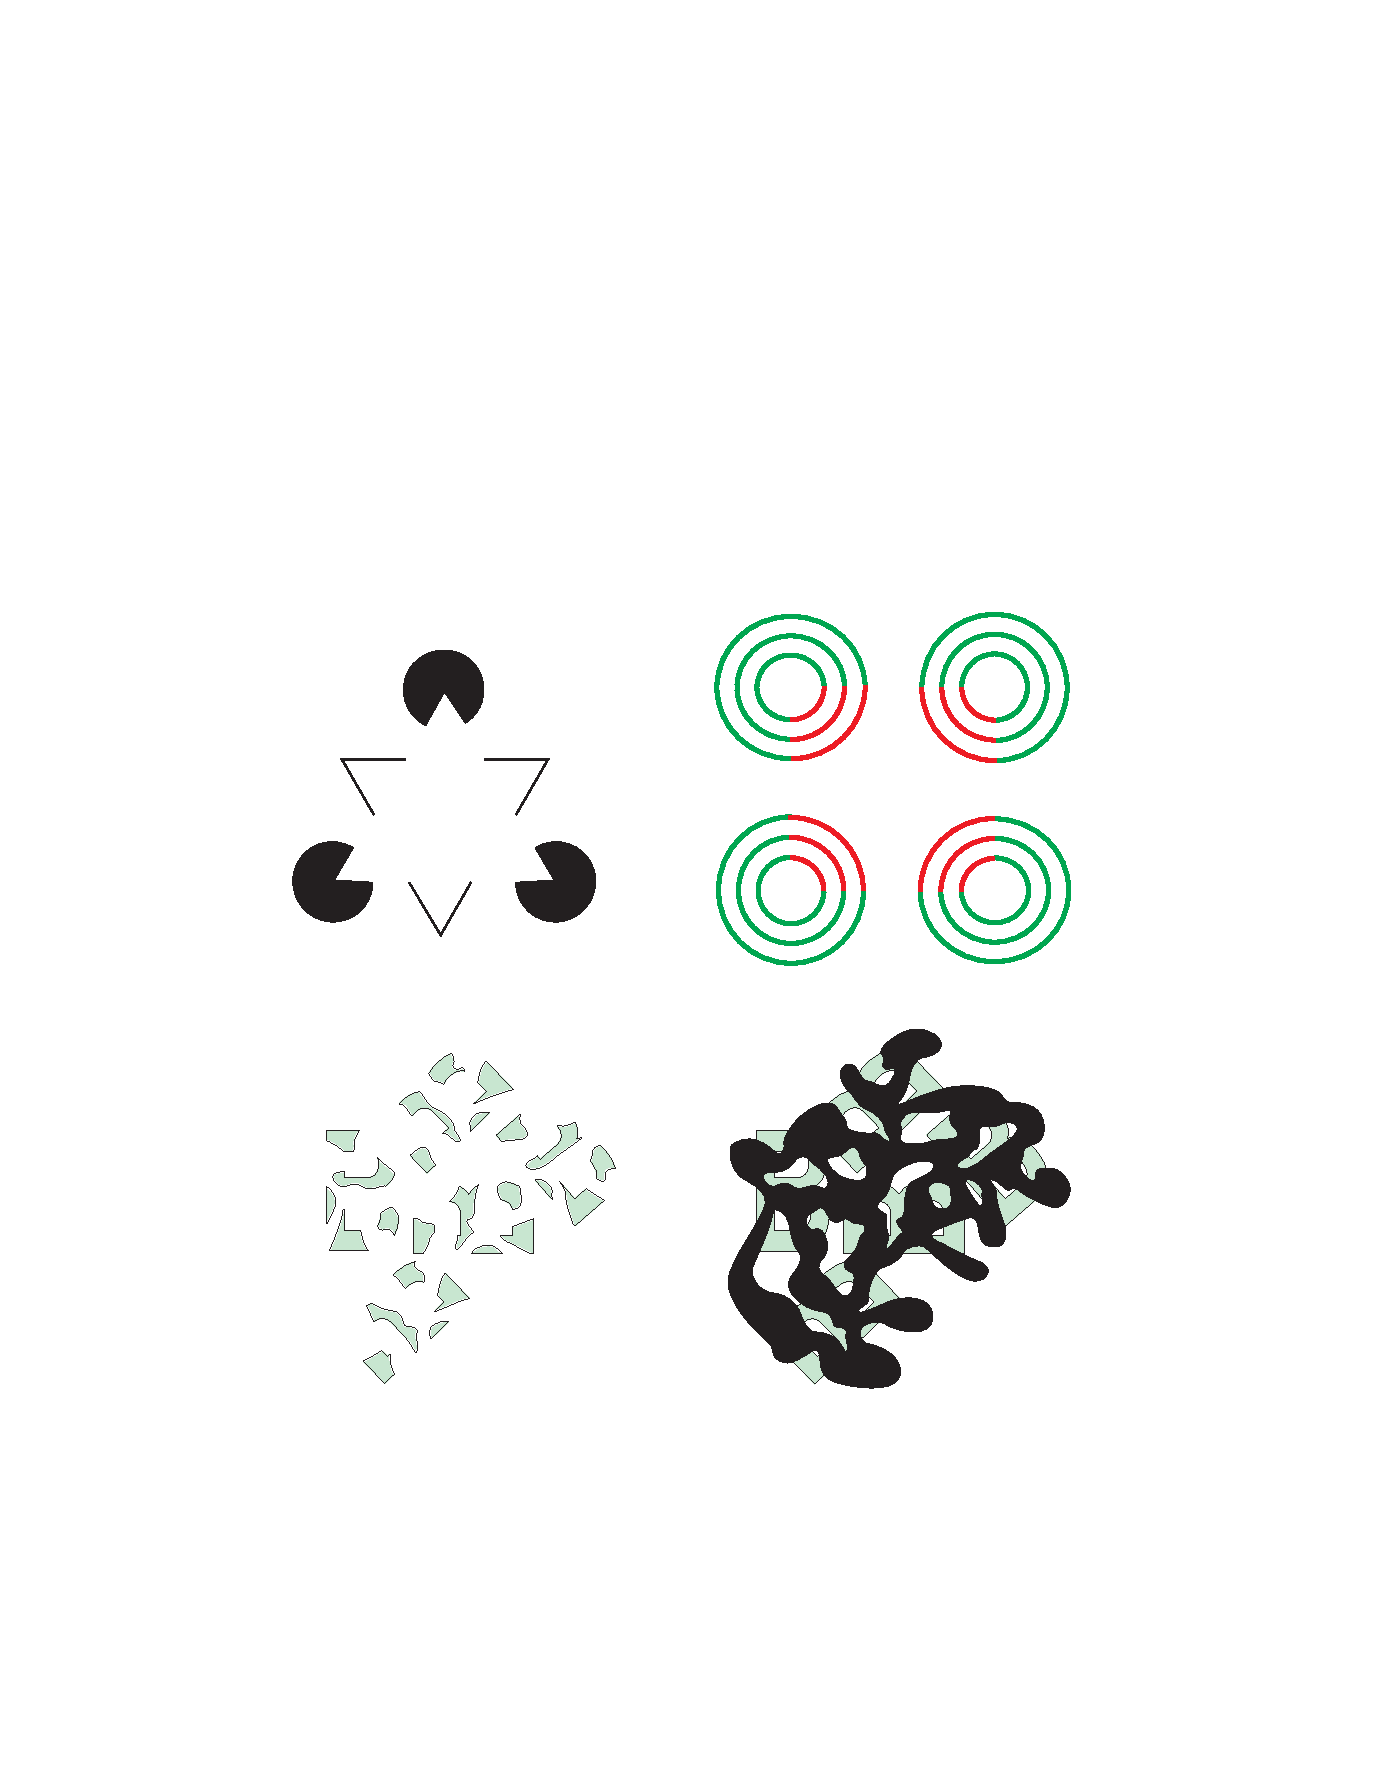
\includegraphics[width=1.0\linewidth]{chap23/fig_23_1}
	\caption{虚幻的轮廓和感性的填充。
		视觉系统使用关于局部方向和对比度的信息来构建物体的轮廓和表面。
		这种建设性的过程可以导致对没有出现在视野中的轮廓和表面的感知,包括在虚幻的图形中看到的轮廓和曲面。
		左上角:在卡尼萨三角形错觉中,人们可以感知到白色三角形顶点之间延伸的连续边界,尽管唯一真正的轮廓元素是由吃豆人形状和锐角形成的。
		右上角:虚幻的粉红色正方形的内部和外部与页面的白色相同,但可以看到正方形内连续的透明粉红色表面。
		底部:遮挡曲面也可以促进轮廓集成和曲面分割。
		左边的不规则形状看起来是不相关的,但当它们被黑色形状(右边)部分遮挡时,它们很容易被视为字母B的碎片。}
	\label{fig:23_1}
\end{figure}


视觉处理的三个特征有助于克服来自视网膜的信号的歧义。
首先,感知视觉特征的方式取决于它周围的一切。
例如,对点、线或表面的感知取决于该特征与场景中存在的其他事物之间的关系。
也就是说,视觉皮层中神经元的反应是依赖于上下文的:
它取决于细胞感受野外的轮廓和表面的存在,以及细胞感受野内的属性。
其次,视觉皮层神经元的功能特性可以通过视觉体验或知觉学习来改变。
最后,皮层中的视觉处理受认知功能的影响,特别是注意力、期望和“感知任务”(积极参与视觉辨别或检测)。
这三个因素(表示场景的上下文或整套信号、皮层回路中经验依赖性变化以及期望)之间的相互作用对于视觉系统对复杂场景的分析至关重要。


在本章中,我们将研究大脑对视觉场景中局部特征或视觉原始要素的分析如何与对更多全局特征的分析并行进行。
视觉原始要素包括对比度、线方向、亮度、颜色、运动和深度。
每种类型的视觉原始要素都受到中间级处理的综合作用。
具有特定方向的线被整合到物体轮廓中,局部对比度信息被整合到表面亮度和表面分割中,波长选择性被整合到颜色恒常性中,方向选择性被整合到物体运动中。


视觉原始要素的分析从视网膜开始,检测亮度和颜色,然后在初级视觉皮层继续分析方位、运动方向和立体深度。
与中层视觉处理相关的属性与从初级视觉皮层开始的视觉皮层中的视觉原始要素一起分析,它在轮廓整合和表面分割中发挥作用。
视觉皮层的其他区域专注于这项任务的不同方面:
V2 分析与物体表面相关的属性,V4 整合关于颜色和物体形状的信息,而 V5(颞中区或\textit{内侧颞叶})整合空间中的运动信号(图~\ref{fig:23_2})。


\begin{figure}[htbp]
	\centering
	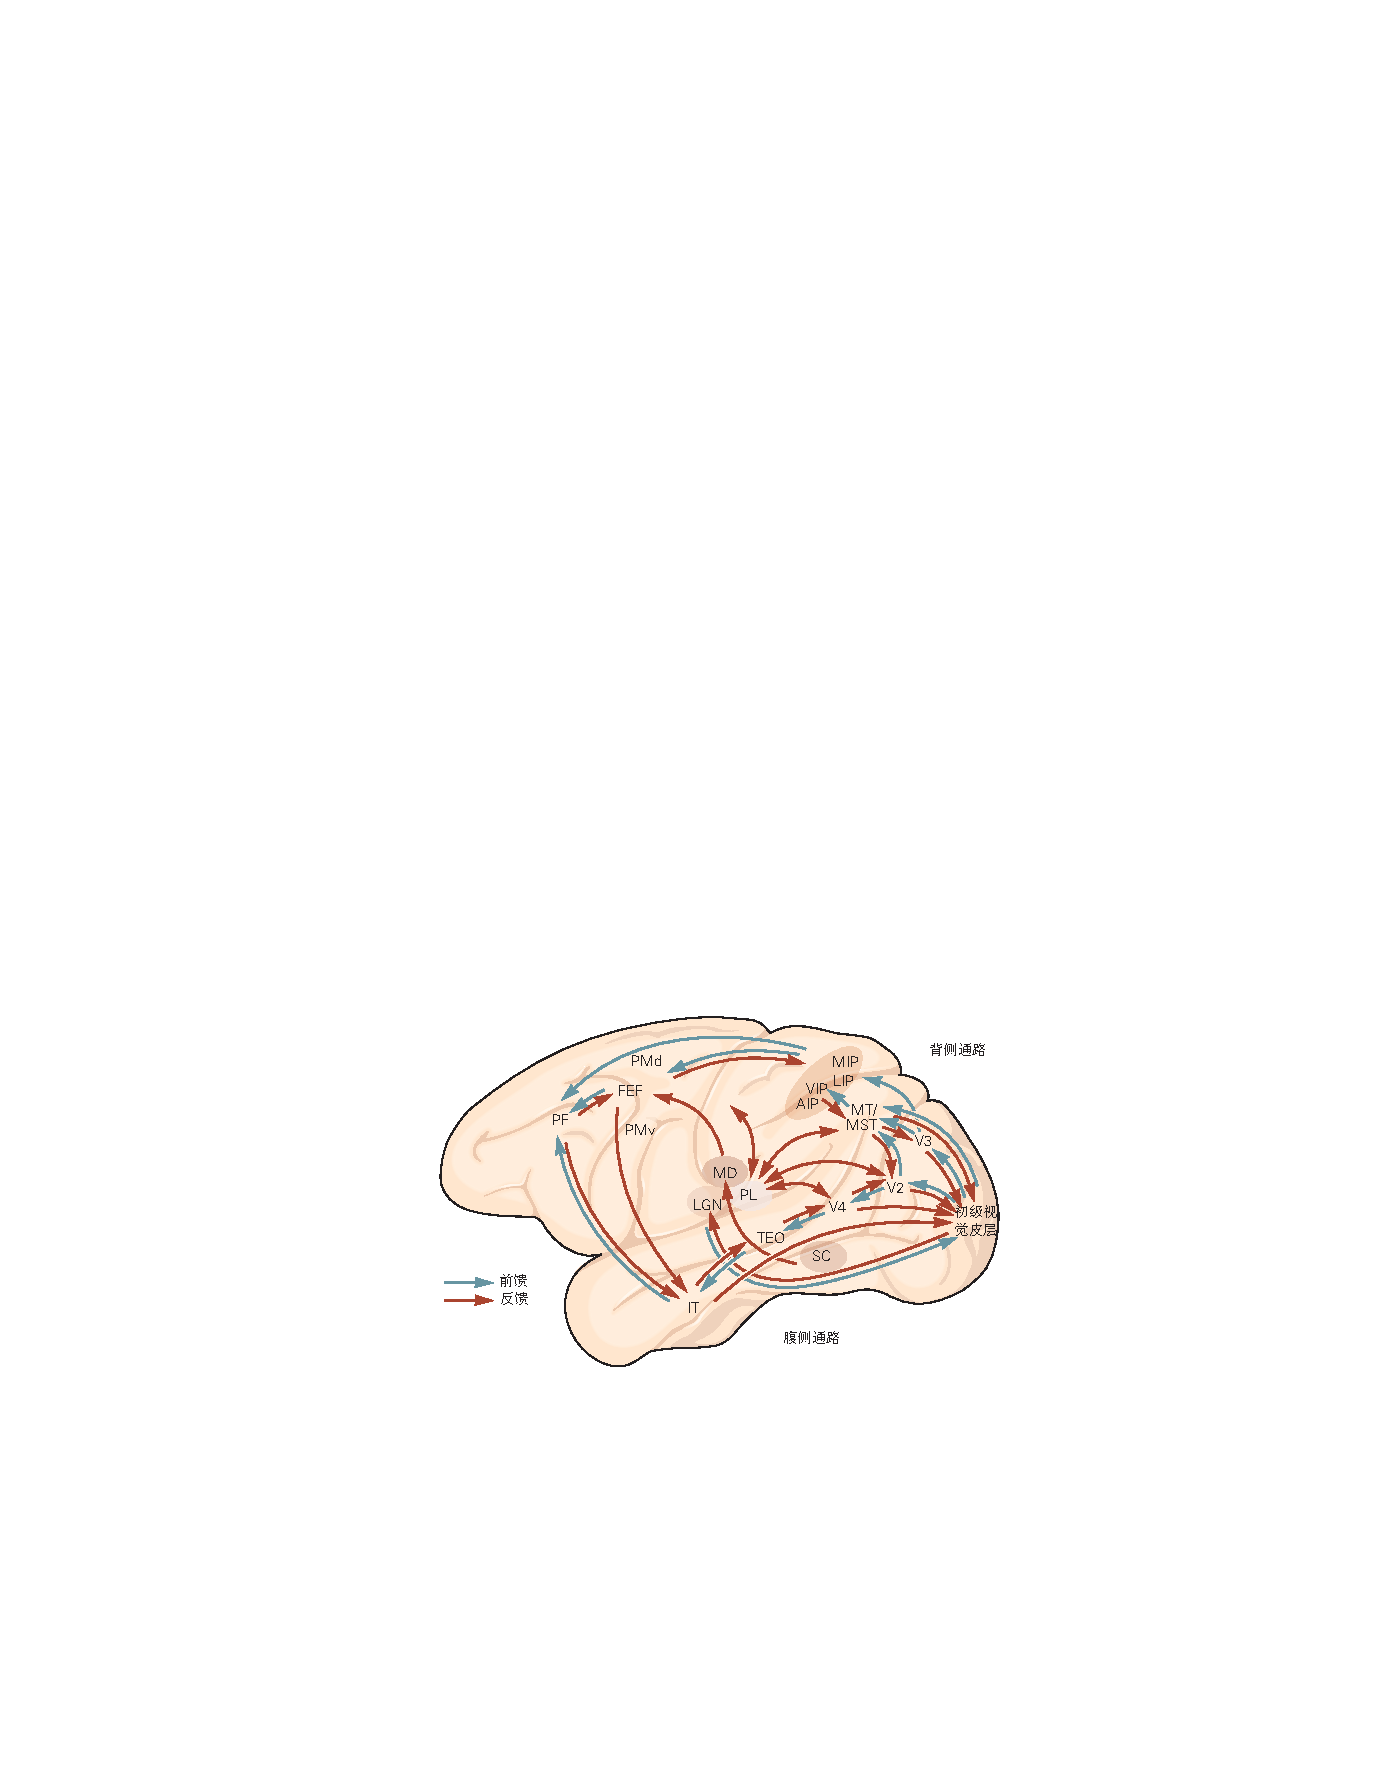
\includegraphics[width=0.8\linewidth]{chap23/fig_23_2}
	\caption{涉及中层水平视觉处理的皮层区域。
		猕猴的许多皮层区域,包括V1、V2、V3、V4和\textit{内侧颞叶},都参与整合局部线索以构建轮廓和表面,并将前景与背景分离。
		阴影区域延伸到额叶和颞叶,因为这些区域的认知输出,包括注意力、期望和行为任务,有助于场景分割过程。}
	\label{fig:23_2}
\end{figure}



\section{物体几何内部模型帮助大脑分析形状}

确定目标轮廓的第一步是识别轮廓局部部分的方向。
此步骤从初级视觉皮层开始,该步骤在局部和全局形式分析中都起着至关重要的作用。


视觉皮层中的神经元对视野的特定局部特征有选择性响应,包括方向,双眼差或深度,运动方向以及在视网膜和外侧膝状核中已经分析的特性,例如对比度和颜色。 
方向选择性,这是1959年\textit{大卫$\cdot$休伯尔}和\textit{托斯坦$\cdot$威泽尔}在皮层神经元的感受野中发现的第一个新兴特性。


视网膜(第~\ref{chap:chap22}~章)和外侧膝状核(第~\ref{chap:chap21}~章)中的神经元都有具有中心周围组织的圆形感受野。
它们响应视野中边缘或线条的光线对比度,但对这些边缘的方向没有选择性(见图~\ref{fig:21_9})。
然而,在视觉皮层中,神经元对特定方向的线有选择性反应。
每个神经元对狭窄的方向响应,大约40°,并且不同的神经元对不同方向的反应最佳。
\textit{休伯尔}和\textit{威泽尔}提出,这种方向选择性反映了从外侧膝状核中输入的排列,现在有大量支持该思想的支持证据。
每个初级视觉皮层神经元都从几个相邻的膝状核神经元中接收输入,这些神经元的中心周围感受野是对齐的,以表示特定的方向轴(图~\ref{fig:23_3})。
已经确定了两种主要的方向选择性神经元的类型。


\begin{figure}[htbp]
	\centering
	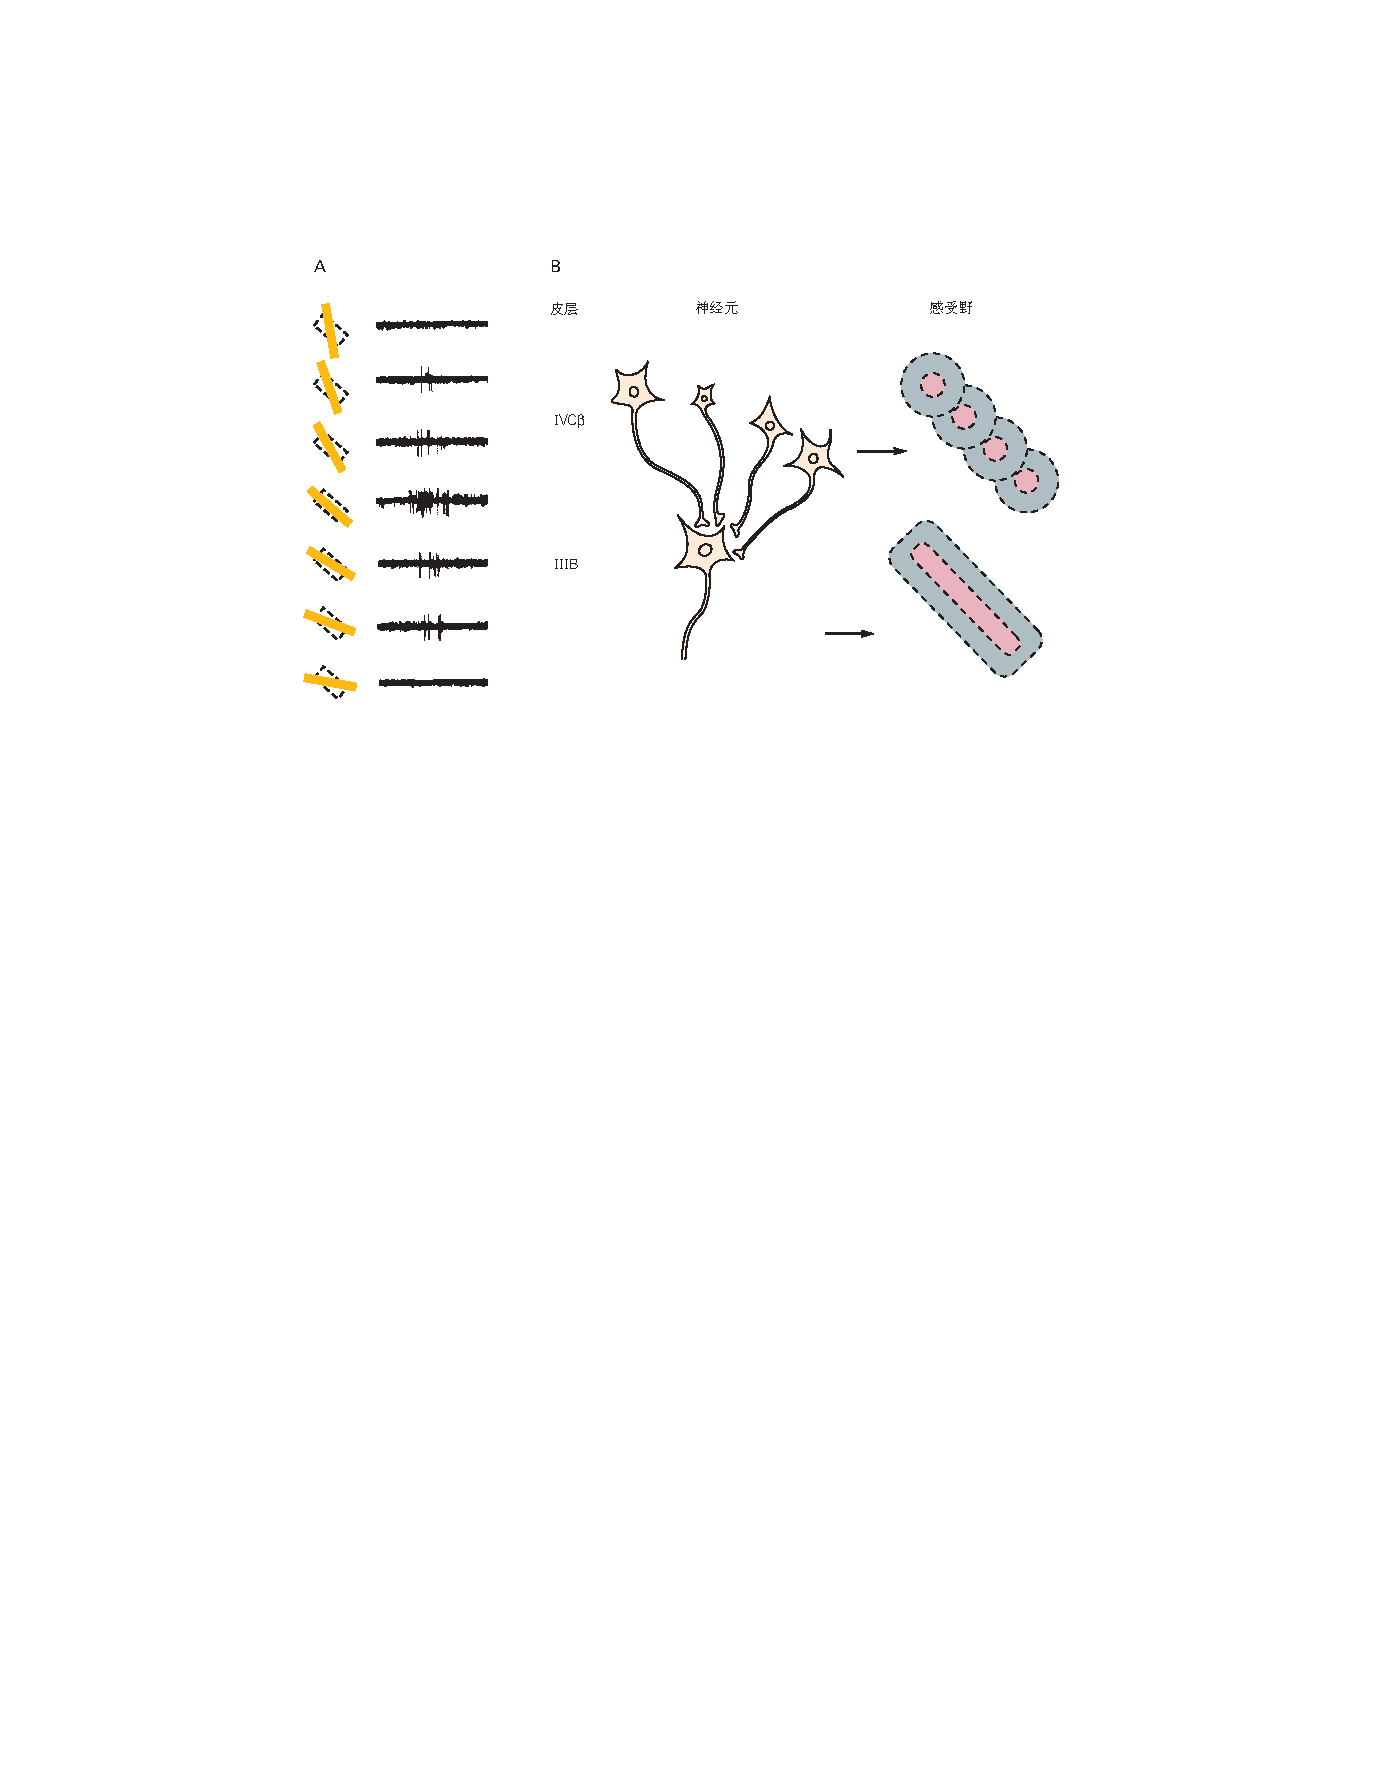
\includegraphics[width=0.95\linewidth]{chap23/fig_23_3}
	\caption{方向选择性和机制。
		\textbf{A.} 初级视觉皮层中的神经元选择性地响应适合其感受野方向的线段。
		这种选择性是大脑分析物体形状的第一步\cite{hubel1968receptive}。
		\textbf{B.} 感受野的方向被认为是由几个突触前细胞的圆形中心-环绕感受野对齐的结果。 
		膝状核。
		在猴子中,初级视觉皮层层 IVC$\beta$ 中的单个神经元具有无方向的感受野。
		然而,当几个相邻的 IVC$\beta$ 细胞投射到 IIIB 层中的神经元时,它们会为该突触后细胞创建一个具有特定方向的感受野。}
	\label{fig:23_3}
\end{figure}


简单细胞的感受野分为ON和OFF子域(图~\ref{fig:23_4})。
当视觉刺激(例如光线)进入感受野的ON子域时,神经元会发放动作电位。
当光条离开OFF子域时,该细胞也会做出响应。
简单细胞对移动光条具有特征性响应。
当一条光条从OFF子域移动到ON子域时,它们会迅速活跃。
因此,这些细胞的反应对于空间中线条或边缘的位置具有很高的选择性。


\begin{figure}[htbp]
	\centering
	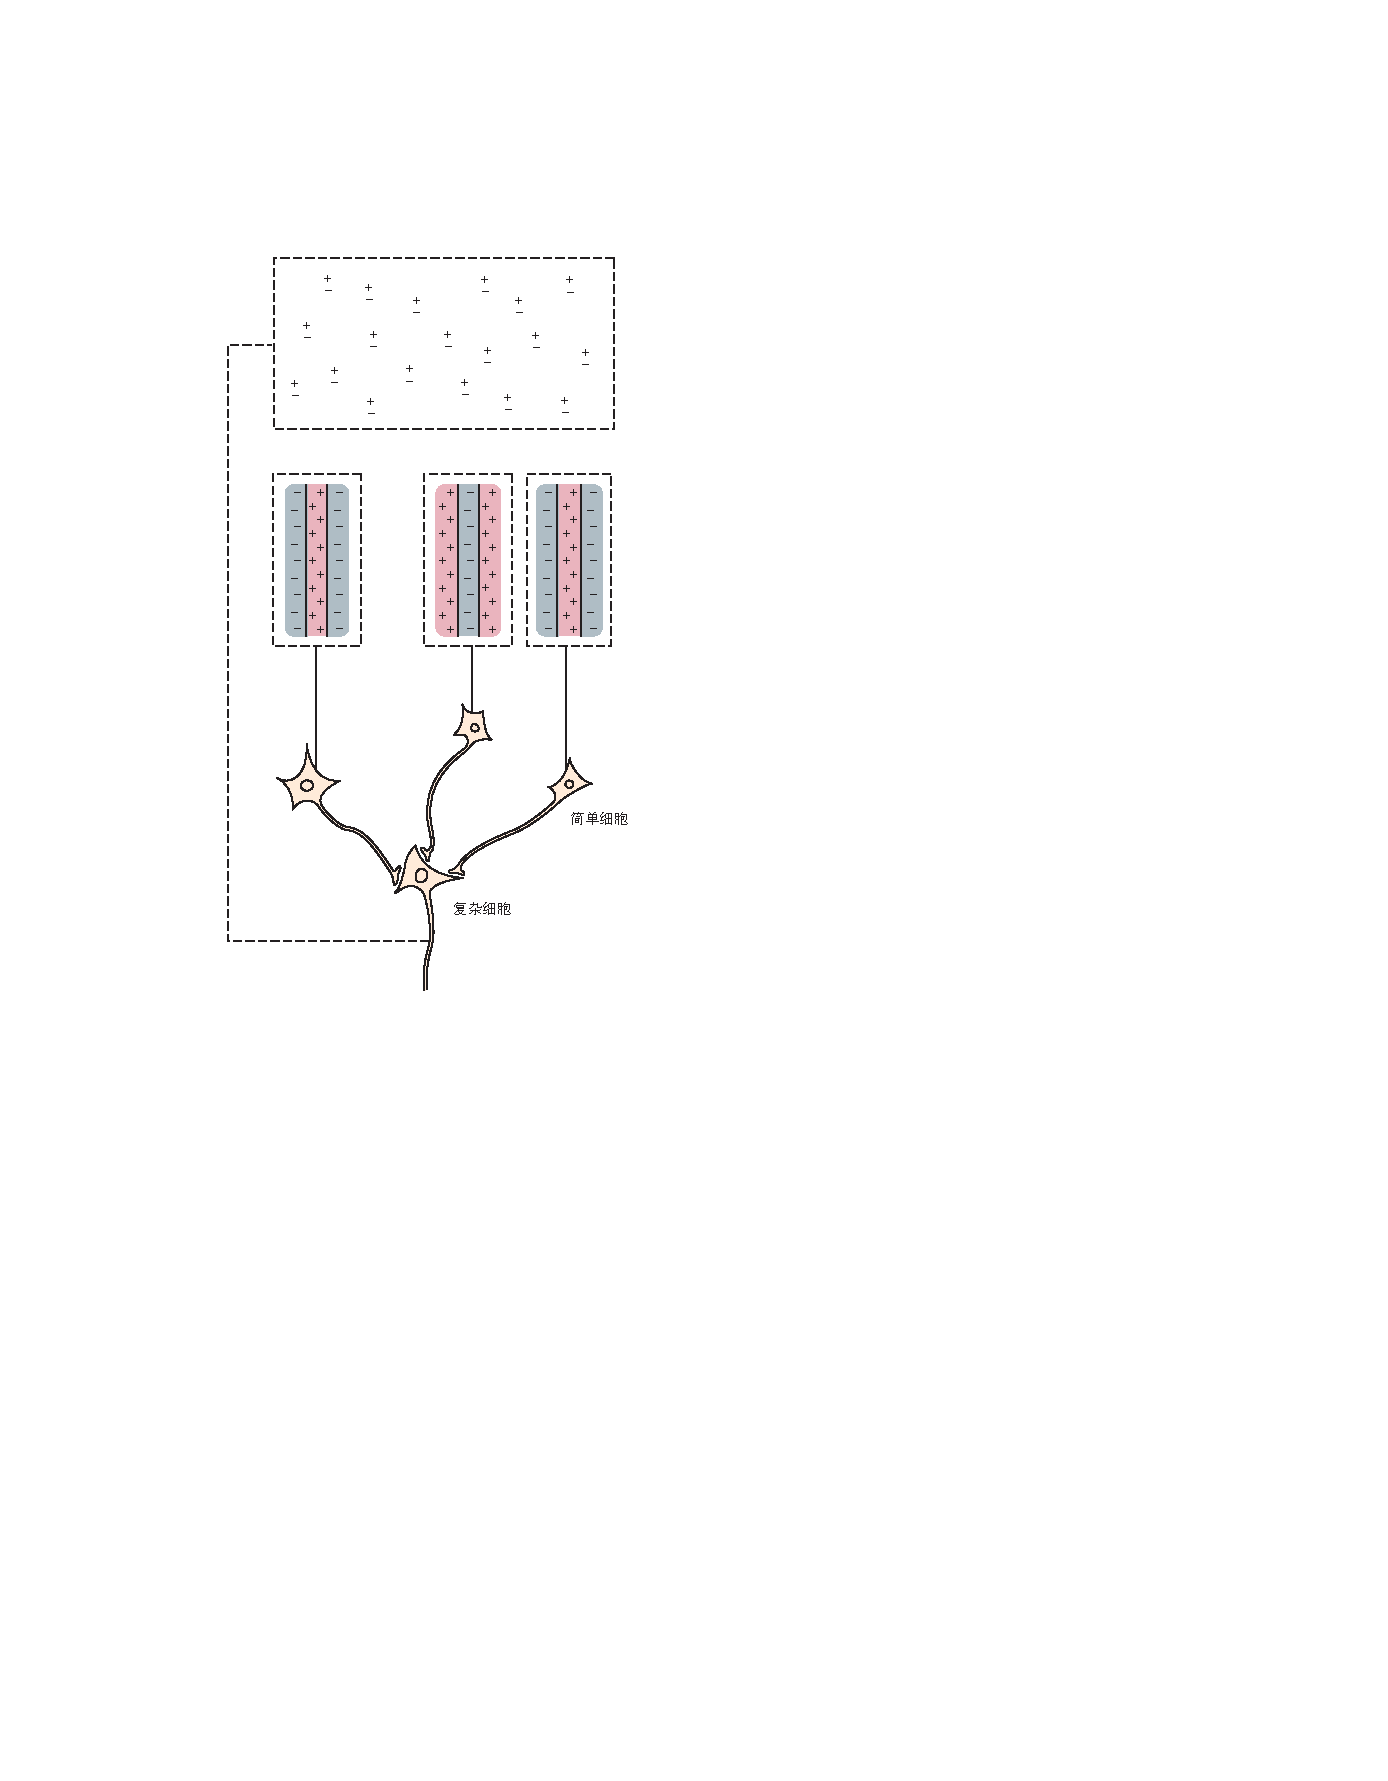
\includegraphics[width=0.6\linewidth]{chap23/fig_23_4}
	\caption{视觉皮层中的简单和复杂细胞。
		简单细胞的感受野被分成具有相反响应特性的子域。
		在\textit{给光}子域(用 + 表示)中,光的开始触发神经元的反应;
		在\textit{撤光}子场(由 - 表示)中,光条的熄灭触发响应。
		复杂细胞具有重叠的ON和OFF区域,并且当线或边缘沿着垂直于感受野方向的轴穿过感受野时连续响应。}
	\label{fig:23_4}
\end{figure}


复杂细胞对目标边界的位置的选择性较小。
他们缺乏明确的ON和OFF子域(图~\ref{fig:23_4}),并且在其感受野的所有位置都对光和暗做出了类似的反应。
他们随着线或边缘刺激的遍历而持续活跃。
\textit{休伯尔}和\textit{威泽尔}提出,复杂的细胞是简单感受野之后阐述的第二阶段,并且是通过重叠的简单感受野构建的。


当人们考虑到早期视皮层区域中描述的感受野特性的范围时,重要的是要指出系统发育的差异,不同物种在这些特性首次表达的位置和表现的特性种类方面存在差异。
在猫的视觉皮层中,外侧膝状核神经元的目标层具有定向的简单细胞。
据推测,这些皮层细胞代表了视觉信息的皮层处理中的一个必要的第一阶段,位于外侧膝状核中心-周围圆对称感受野和皮层表浅层复杂细胞的感受野之间。
然而,在灵长类动物中,膝状核的目标层4C$\alpha$和$\beta$具有圆形的对称,无定向的接受场。
4C层细胞的后突触靶主要是皮层的表层,并用复杂的细胞填充,因此跳过了一个简单的细胞阶段。
在小鼠中,在外侧膝状核中可以看到方向选择性。
前面的比较指出了视觉处理演变的一些特征。
一个是功能的脑化,其中诸如方向之类的属性转移到了进化阶段的处理阶段。
另一个是新途径的发展。
有人提出,灵长类动物的大细胞通路相当于猫的整个膝状纹状体通路,而小细胞通路,介导更高分辨率的视觉和彩色视觉,对灵长类动物是新的。


运动刺激通常用于研究视觉皮层神经元的感受野,不仅用于模拟检测到空间中的物体在空间中移动的条件,还可以模拟眼睛运动产生的条件。
当我们扫描视觉环境时,静止物体的边界会在视网膜上移动。
实际上,视觉感知需要眼动。
视觉皮层神经元对在视网膜上稳定的图像没有反应。
这些神经元需要瞬时刺激(移动或闪烁刺激)才能激活。


一些视觉皮层神经元具有感受野,其中兴奋中心的两侧是抑制区域。
沿着方向轴的抑制区域(即所谓的末端抑制性)限制了神经元对一定长度线的响应(图~\ref{fig:23_5})。
末端抑制性神经元对不延伸到抑制性区域但完全位于兴奋性部分的感受野内的线条响应很好。
由于抑制区具有中央兴奋性区域的取向偏好,因此末端抑制性细胞对线曲率有选择性,并且对角的反应也很好。


\begin{figure}[htbp]
	\centering
	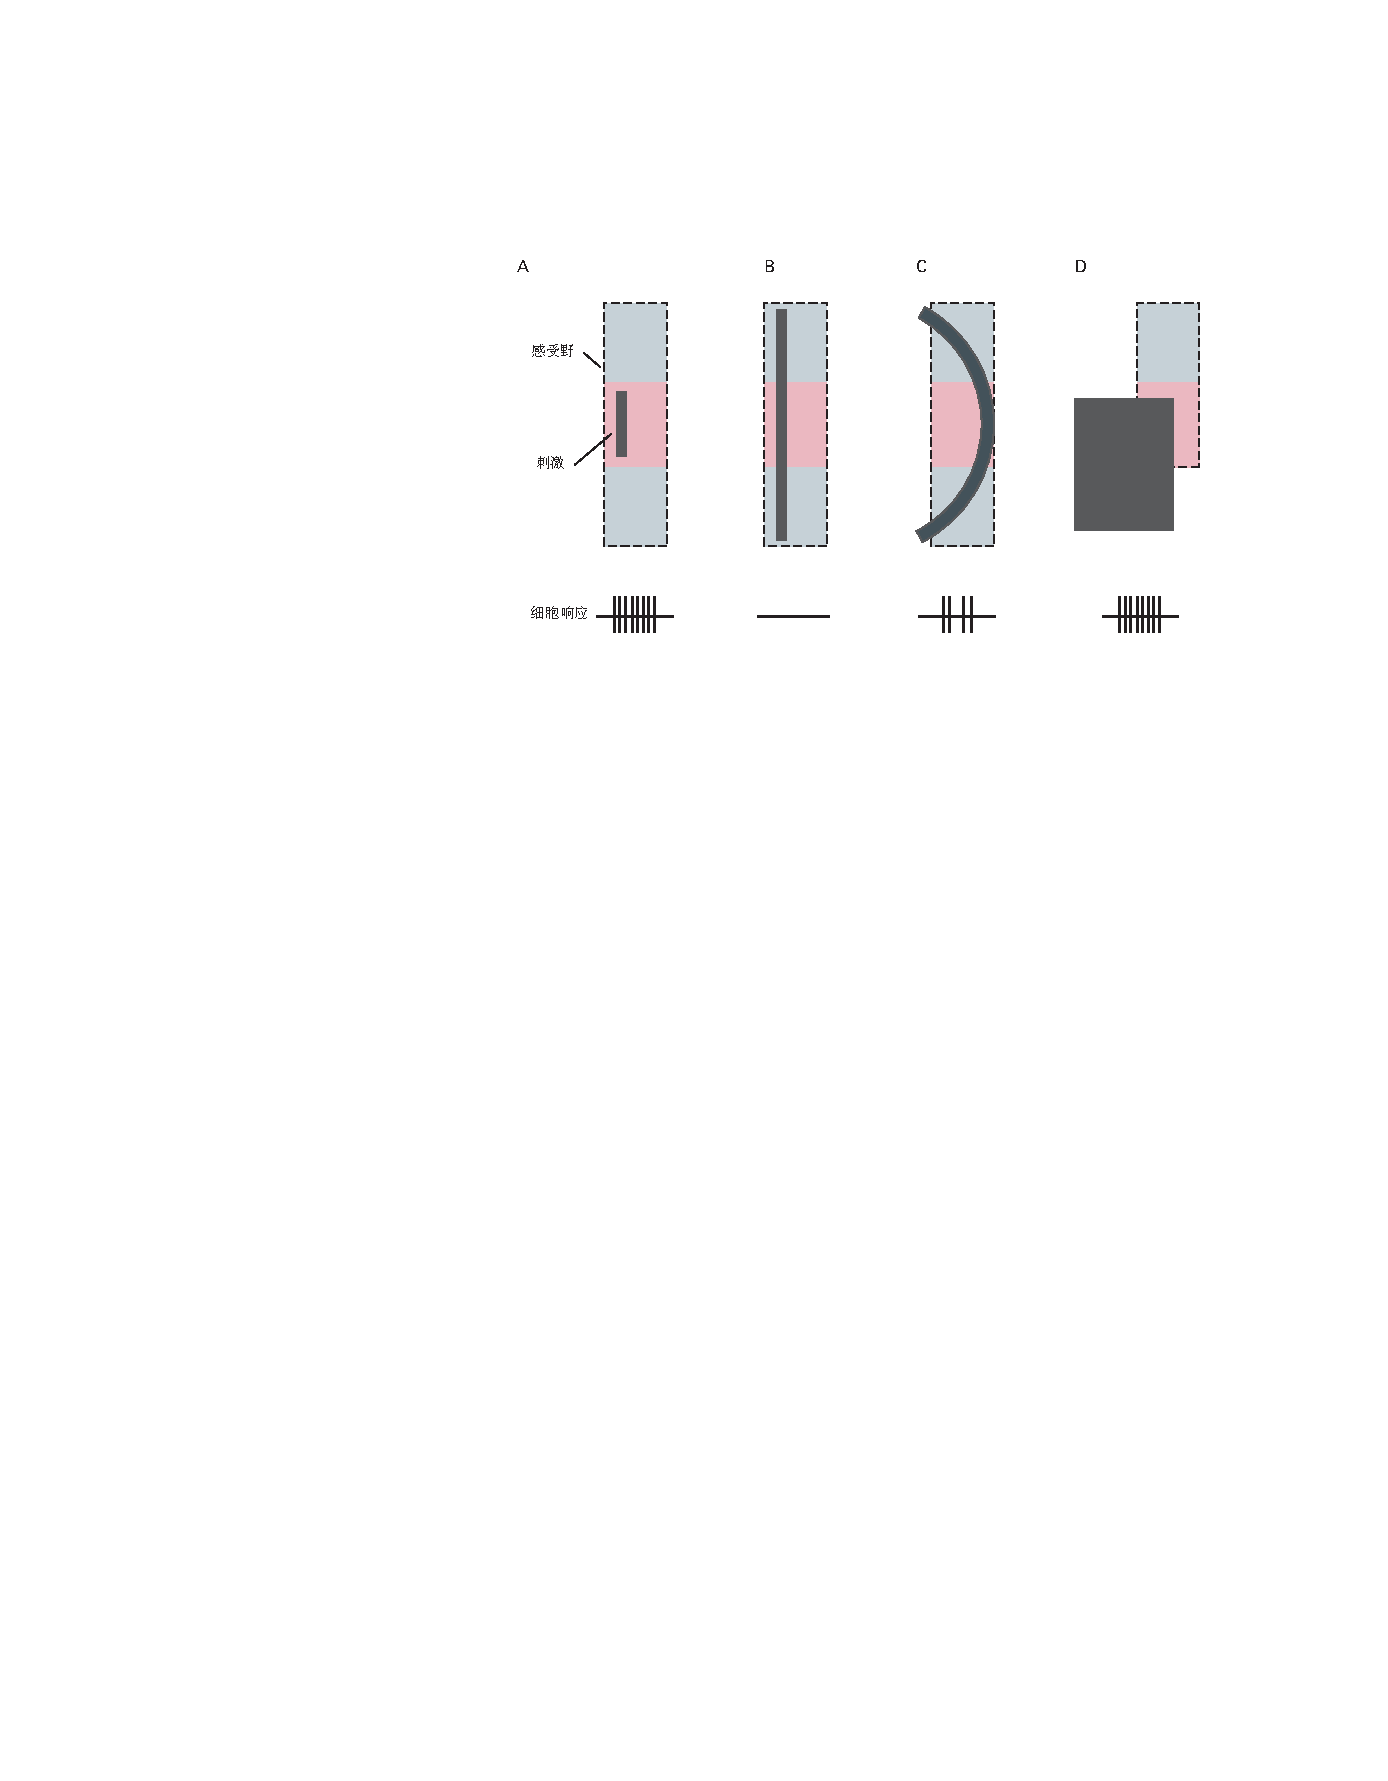
\includegraphics[width=0.85\linewidth]{chap23/fig_23_5}
	\caption{末端抑制感受野。
		一些感受野有一个中央兴奋区,两侧是具有相同方向选择性的抑制区。因此,短线段或长曲线将激活神经元(A 和 C),但长直线不会(B)。
		具有感受野的神经元除兴奋区外仅显示一个抑制区,可以发出角点(D)存在的信号。}
	\label{fig:23_5}
\end{figure}


为了定义整个目标的形状,视觉系统必须将有关局部方向和曲率的信息集成到目标轮廓中。
视觉系统整合轮廓的方式反映了自然世界中存在的几何关系(图~\ref{fig:23_6})。
正如格式塔心理学家最初在20世纪初指出的那样,立即识别的轮廓往往遵循良好的延续规则(弯曲线保持稳定的曲率半径和直线的持续性)。
在复杂的视觉场景中,这种光滑的轮廓往往会“弹出”,而更多的锯齿状轮廓很难检测到。


\begin{figure}[htbp]
	\centering
	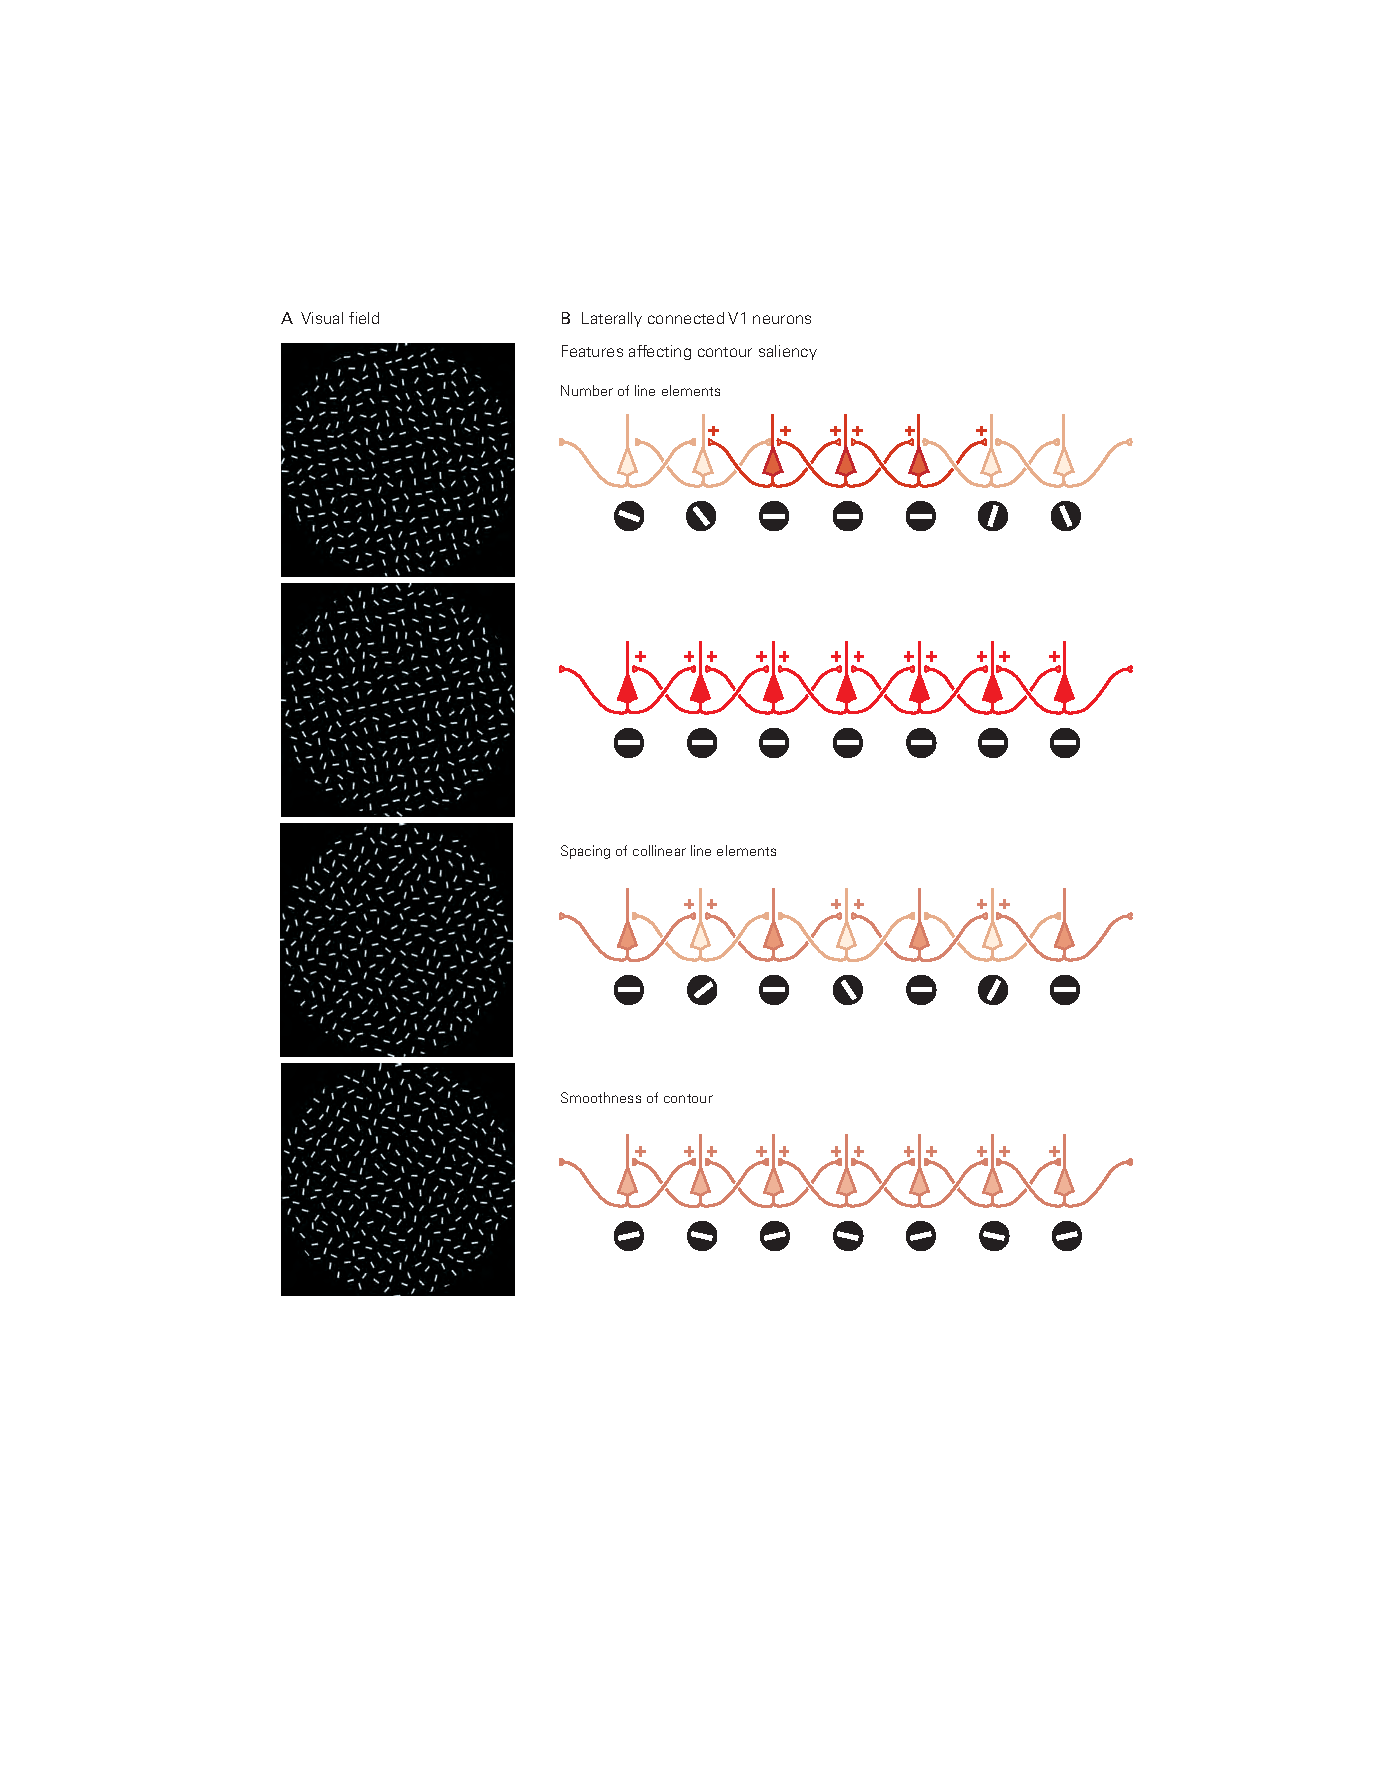
\includegraphics[width=1.0\linewidth]{chap23/fig_23_6}
	\caption{轮廓整合反映了接近和良好连续的感知规则\cite{li2002global}。
		\textbf{A.} 一条直线由一个或多个具有相同倾斜方向的轮廓元素组成,出现在此处四个图像中每一个的中心。
		在某些图像中,线条或多或少会立即弹出,无需搜索。
		影响轮廓显著性的因素包括轮廓元素的数量(比较第一帧和第二帧)、元素间距(第三帧)和轮廓的平滑度(底部帧)。
		当元素之间的间距太大或它们之间的方向差异太大时,必须搜索图像以找到轮廓。
		\textbf{B.} 这些感知特性反映在具有相似方向选择性的初级视觉皮层神经元柱之间的水平连接中。
		只要视觉元素之间的距离足够近,兴奋就可以从一个细胞传播到另一个细胞,从而促进初级视觉皮层神经元的反应。
		然后,网络中的每个神经元都会增强任一侧神经元的响应,并且促进的响应会在整个网络中传播。}
	\label{fig:23_6}
\end{figure}


视觉皮层神经元的反应可以通过刺激来调节,刺激本身不会激活细胞,因此位于接受场的核心之外。
该上下文调节赋予神经元具有更复杂刺激的选择性,而不是通过将刺激的成分放置在接受场和周围的不同位置来预测的。
相同的视觉特征,可以促进复杂场景中目标检测(图~\ref{fig:23_6}a)也适用于上下文调制。
赋予轮廓感感知的特征的特性,甚至是虚幻的特征,都反映在主要视觉皮层中神经元的响应中,这些神经元对轮廓的全局特征敏感,甚至那些延伸在其接受场之外的轮廓。


视觉空间大区域的上下文影响可能是由具有相似方向选择性的视觉皮层中多个神经元之间的连接介导的(图~\ref{fig:23_6}b)。
这些连接是由平行于皮层表面的锥体轴突形成的(见图~\ref{fig:21_16})。
这些水平连接的程度和方向依赖性提供了可以介导轮廓显著性的相互作用(见图~\ref{fig:21_14})。


轮廓整合过程的核心是关联区域的思想。
关联字段是指感知将轮廓元素链接到全局轮廓所需的视觉空间之间的交互。
它奠定了良好延续的格式塔原理,以及嵌入复杂场景中的平滑轮廓的感知显著性。
从生理上讲,它是通过在其“经典”接受场之外延伸的轮廓元素来促进神经元反应的基础。
从解剖学上讲,它部分是由远程水平连接与皮层功能体系结构之间的关系所介导的。
尽管在主要视觉皮层中对其进行了最广泛的研究,但由于皮层所有区域的水平连接无处不在,因此它很可能是关联每个皮层区域中映射的信息位的策略。
缔合场在初级视觉皮层以外的皮层区域的功能作用取决于信息在皮层表面的映射以及这些地图与水平连接丛之间的关系。



\section{深度感知有助于将物体与背景分离}

深度是确定目标感知形状的另一个关键特征。
深度感知的一个重要线索是两只眼睛对世界的看法之间的差异,必须由大脑计算和调和。
双眼输入的整合始于主要视觉皮层,这是单个神经元从两只眼睛接收信号的第一级。
在初级视觉皮层中的细胞中,两只眼睛的输入的平衡(一种称为眼优势)的平衡各不相同。


许多视觉皮层区域中的双眼神经元也是深度的选择性,这是根据位于与观察者不同距离的物体的相对视网膜位置计算得出的。
位于固定平面的目标会在两个视网膜上的相应位置产生图像(图~\ref{fig:23_7})。
位于固定平面前或后面的物体的图像落在两只眼睛的略有不同位置,这是一种被称为双眼差异的特性。
单个神经元可以选择狭窄的差异范围,因此可以深入位置。
有些是对位于固定平面上的物体(调谐兴奋性或抑制性细胞)的选择性,而另一些物体仅当物体位于固定平面(靠近细胞)或该平面后面(远处)时才响应。


\begin{figure}[htbp]
	\centering
	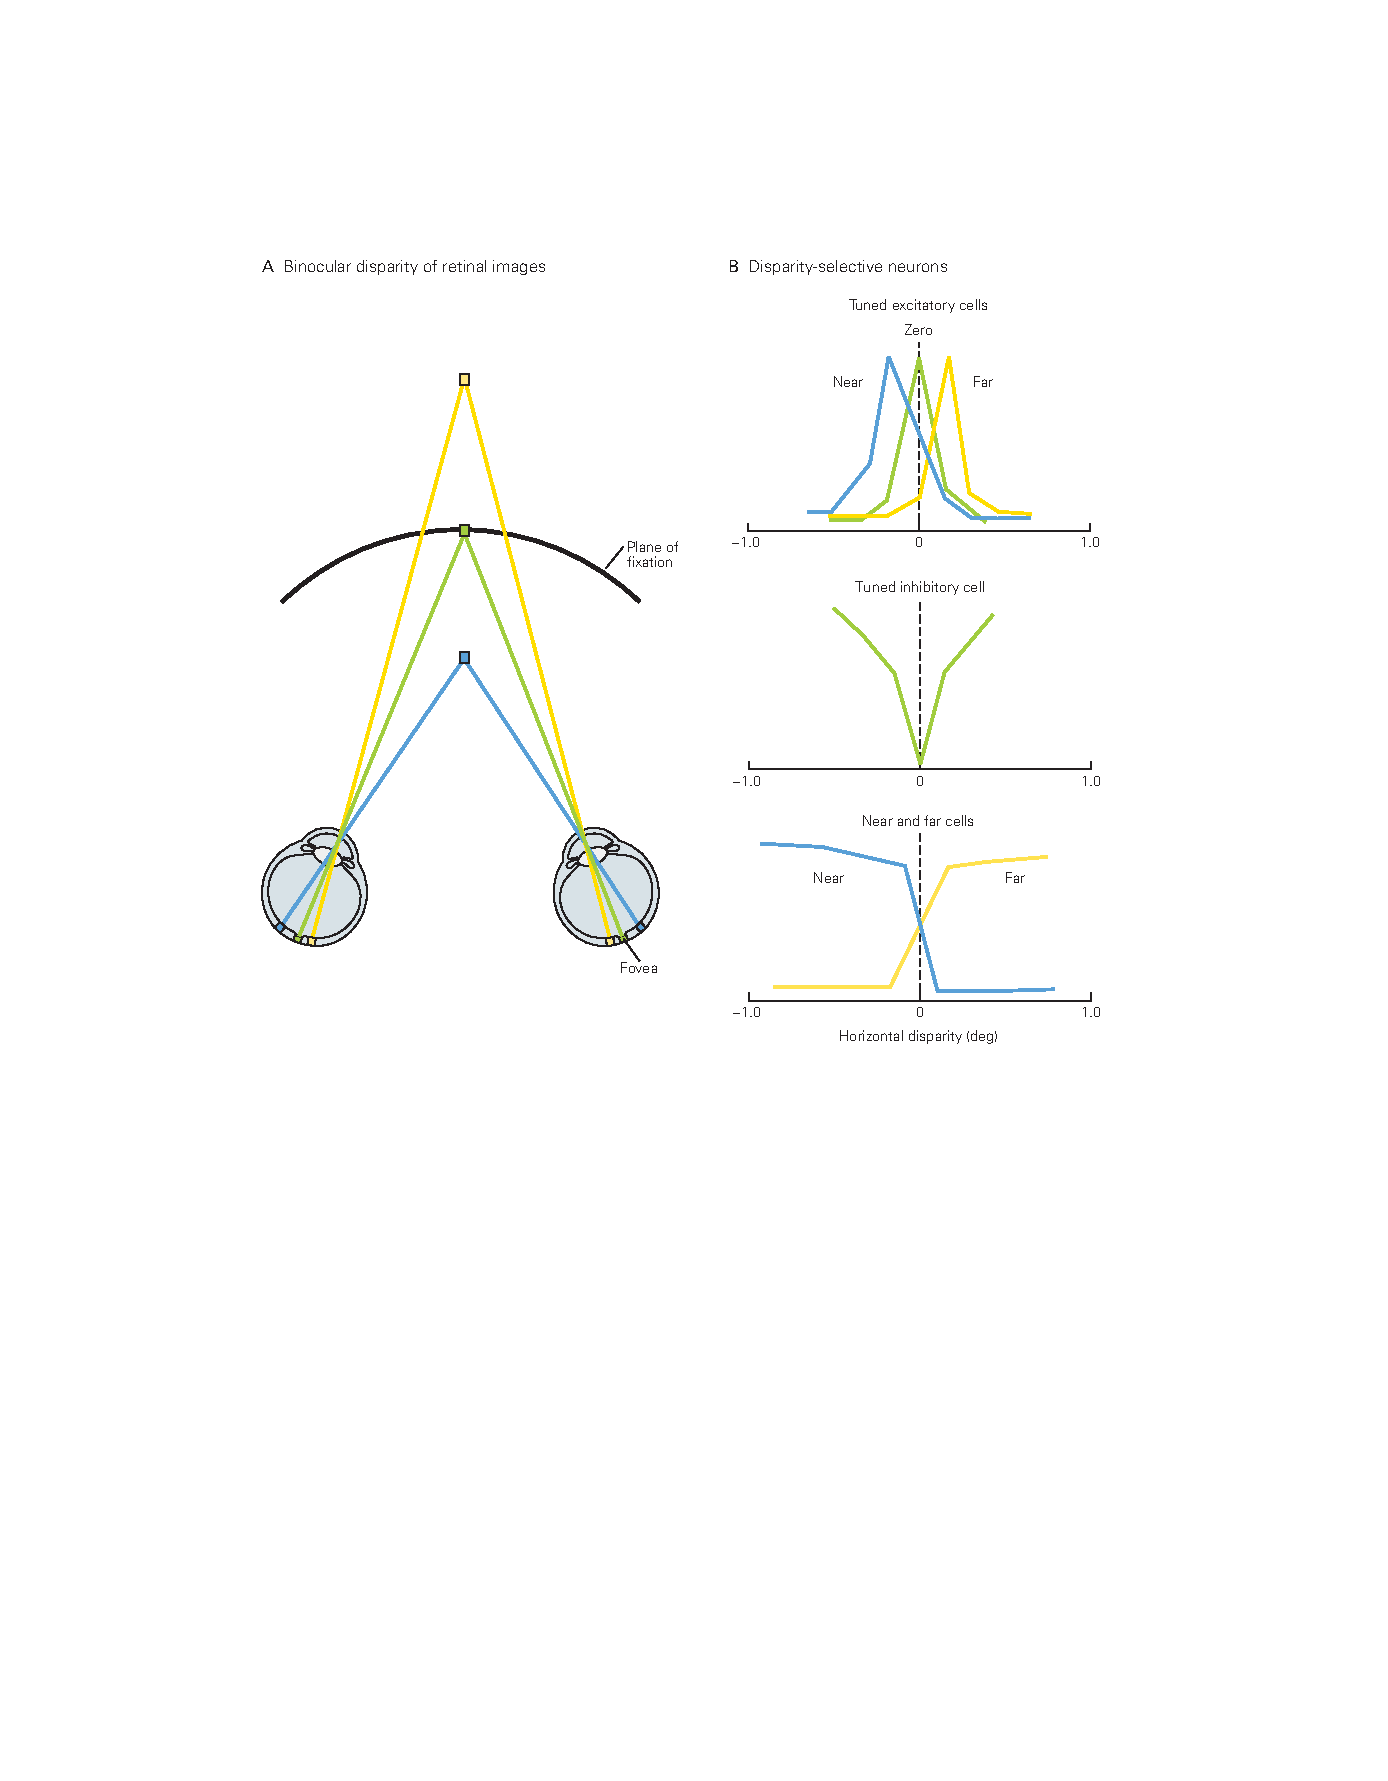
\includegraphics[width=1.0\linewidth]{chap23/fig_23_7}
	\caption{立体视觉和双眼视差。
		\textbf{A.} 深度是根据图像在两只眼睛中出现的位置计算的。
		位于固定平面(绿色)中的物体的图像落在两个视网膜上的相应点上。
		位于固定平面前面(蓝色)或后面(黄色)的物体的图像落在两个视网膜上的不对应位置,这种现象称为双眼视差。
		\textbf{B.} 许多视觉皮层区域的神经元对特定的视差范围具有选择性。
		每个图显示神经元对具有不同视差(横坐标)的双眼刺激的反应。
		一些神经元被调谐到一个狭窄的差异范围,因此具有特定的差异偏好(调谐兴奋性或调谐抑制性神经元),而其他神经元则针对固定平面(近细胞)或平面外(远细胞\footnote{对远像差敏感})前面的物体进行广泛调整\cite{poggio1995mechanisms}}
	\label{fig:23_7}
\end{figure}



深度在目标形状,表面分割以及建立场景的三维特性中起着重要作用。
放置在观察者附近的物体可以部分阻塞那些位于较远的地方。
即使在每个视网膜上的二维图像代表封闭器分隔的两个表面,也将传递在物体后面的表面被认为是连续的。
当大脑遇到被带有适当对准和对比的间隙中断的表面,并位于近深处的平面中时,它填补了间隙以形成连续的表面(图~\ref{fig:23_8})。


\begin{figure}[htbp]
	\centering
	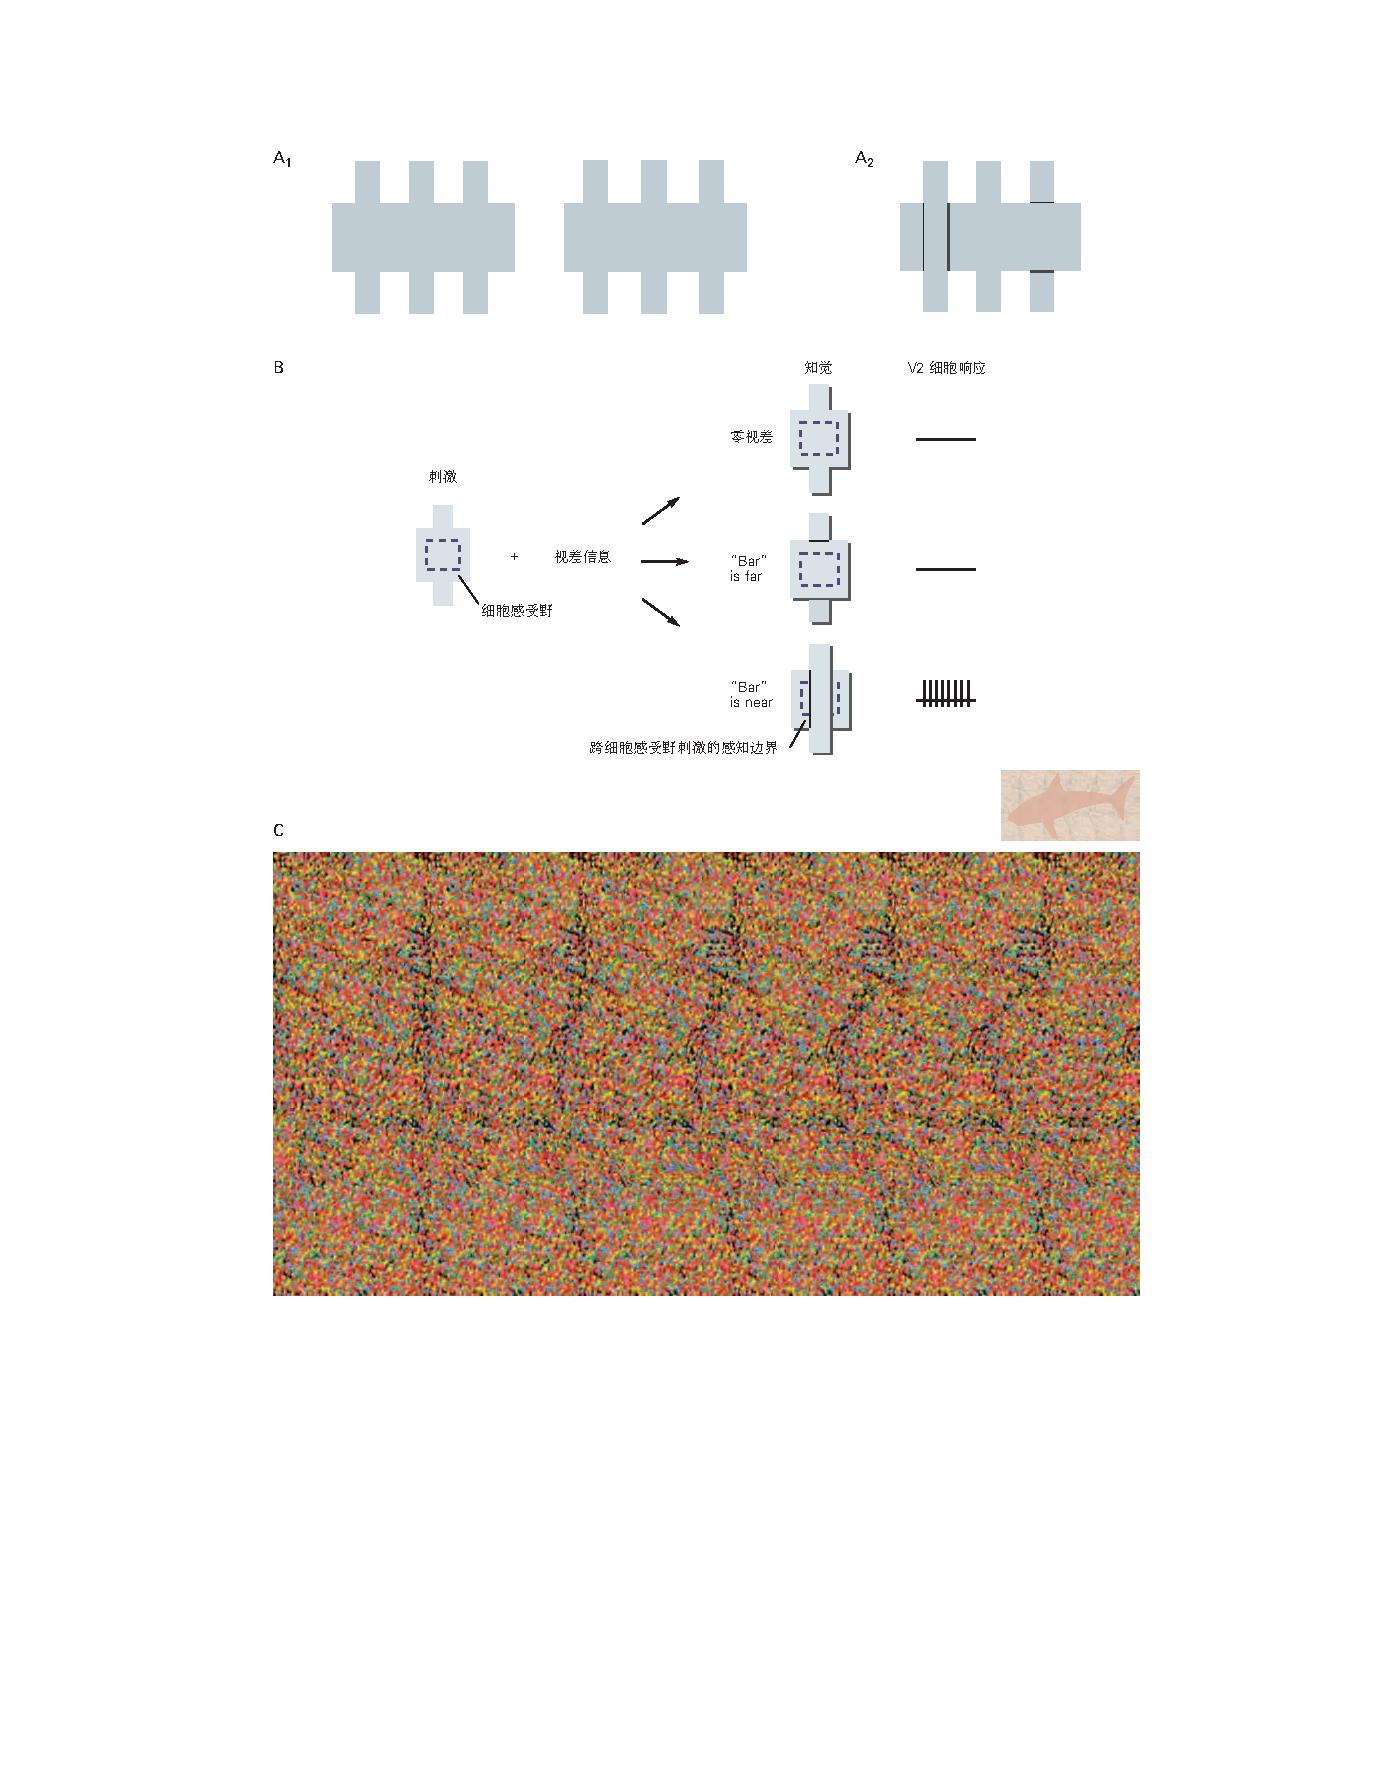
\includegraphics[width=0.95\linewidth]{chap23/fig_23_8}
	\caption{双眼视差的全局分析。
		\textbf{A.} 1. 深度线索有助于表面分割。
		如果您查看三个灰色垂直条穿过灰色水平矩形的图像之一,您会在矩形内看到一个均匀的灰色区域。
		2. 然而,如果你融合两个眼睛发散的矩形,三个垂直条落在两个视网膜上,视差为近、零和远。
		这样看,左边的条形图似乎悬停在矩形前面,有一条虚幻的垂直边缘穿过矩形,而右边的条形图似乎位于水平矩形边缘的后面。
		\textbf{B.} V2 区的神经元对双眼视差线索形成的虚幻边缘做出反应。
		当细胞的感受野以灰色正方形为中心时,细胞不响应与正方形有远差异或相同差异的垂直条。
		当垂直条具有接近差异时,细胞会在虚幻的垂直边缘穿过其感受野时做出反应\cite{bakin2000visual}。
		\textbf{C.} 随机点立体图被视为彩色点的随机阵列,直到你的眼睛发散或会聚,使相邻的深色垂直条纹对齐,产生从背景中出现的鲨鱼的三维图像。
		这种效应源于所选点集的系统差异。}
	\label{fig:23_8}
\end{figure}


尽管可以轻松建立一个目标的深度,但是确定场景中多个目标的深度是一个更复杂的问题,需要将两只眼中所有对象的视网膜图像链接起来。
因此,差异计算是一个全局:视觉图像的一个部分的计算会影响其他部分的计算。
当深度分配在图像的一个部分中是明确的,该信息将应用于图像的其他部分,那里的信息不足以确定深度,这是一种称为差异捕获的现象。


随机点立体图为全局差异分析范围提供了戏剧性的证明。
显示给每只眼睛的视觉信息似乎是不连贯的,但是当立体图被双眼查看时,两个图像中的点随机阵列之间的差异允许嵌入形状可见(图~\ref{fig:23_8}C)。
此感知为基础的计算并不简单,但需要确定左眼显示的哪些功能对应于右眼看到的特征,并在整个图像中传播局部差异信息。


V2区域中的神经元表现出对全球差异提示的敏感性。 
远处的深度提示可用于链接属于目标的轮廓元素,并将它们与目标背景区分开(图~\ref{fig:23_8}B)。


除了双眼差异外,视觉系统还使用许多单眼线索来区分深度。
通过单眼线索的深度确定,例如大小,透视,遮挡,亮度和运动,并不困难。
另一个起源于视觉系统之外的线索是会聚,即不同距离物体的双眼光轴之间的角度。
另一种被称为达立体视觉的双眼线索是一只眼睛可见但被另一只眼睛遮挡的特征。


初级视觉皮层和V2区域中的神经元也表示前景 - 背景关系。
即使该表面的边界远离感受野的边界,在较大表面内具有感受野中心的细胞也可能响应。
这种响应有助于区分目标的背景。
在理解图像时,大脑必须确定哪个边缘属于哪个目标并将每个目标的边缘与背景区分开。 
V2区域中的某些单元具有“边框所有权”的属性,仅在图形而不是背景的情况下触发,即使在两种情况下局部边缘信息相同时,也是对边缘的一侧(图~\ref{fig:23_9})。


\begin{figure}[htbp]
	\centering
	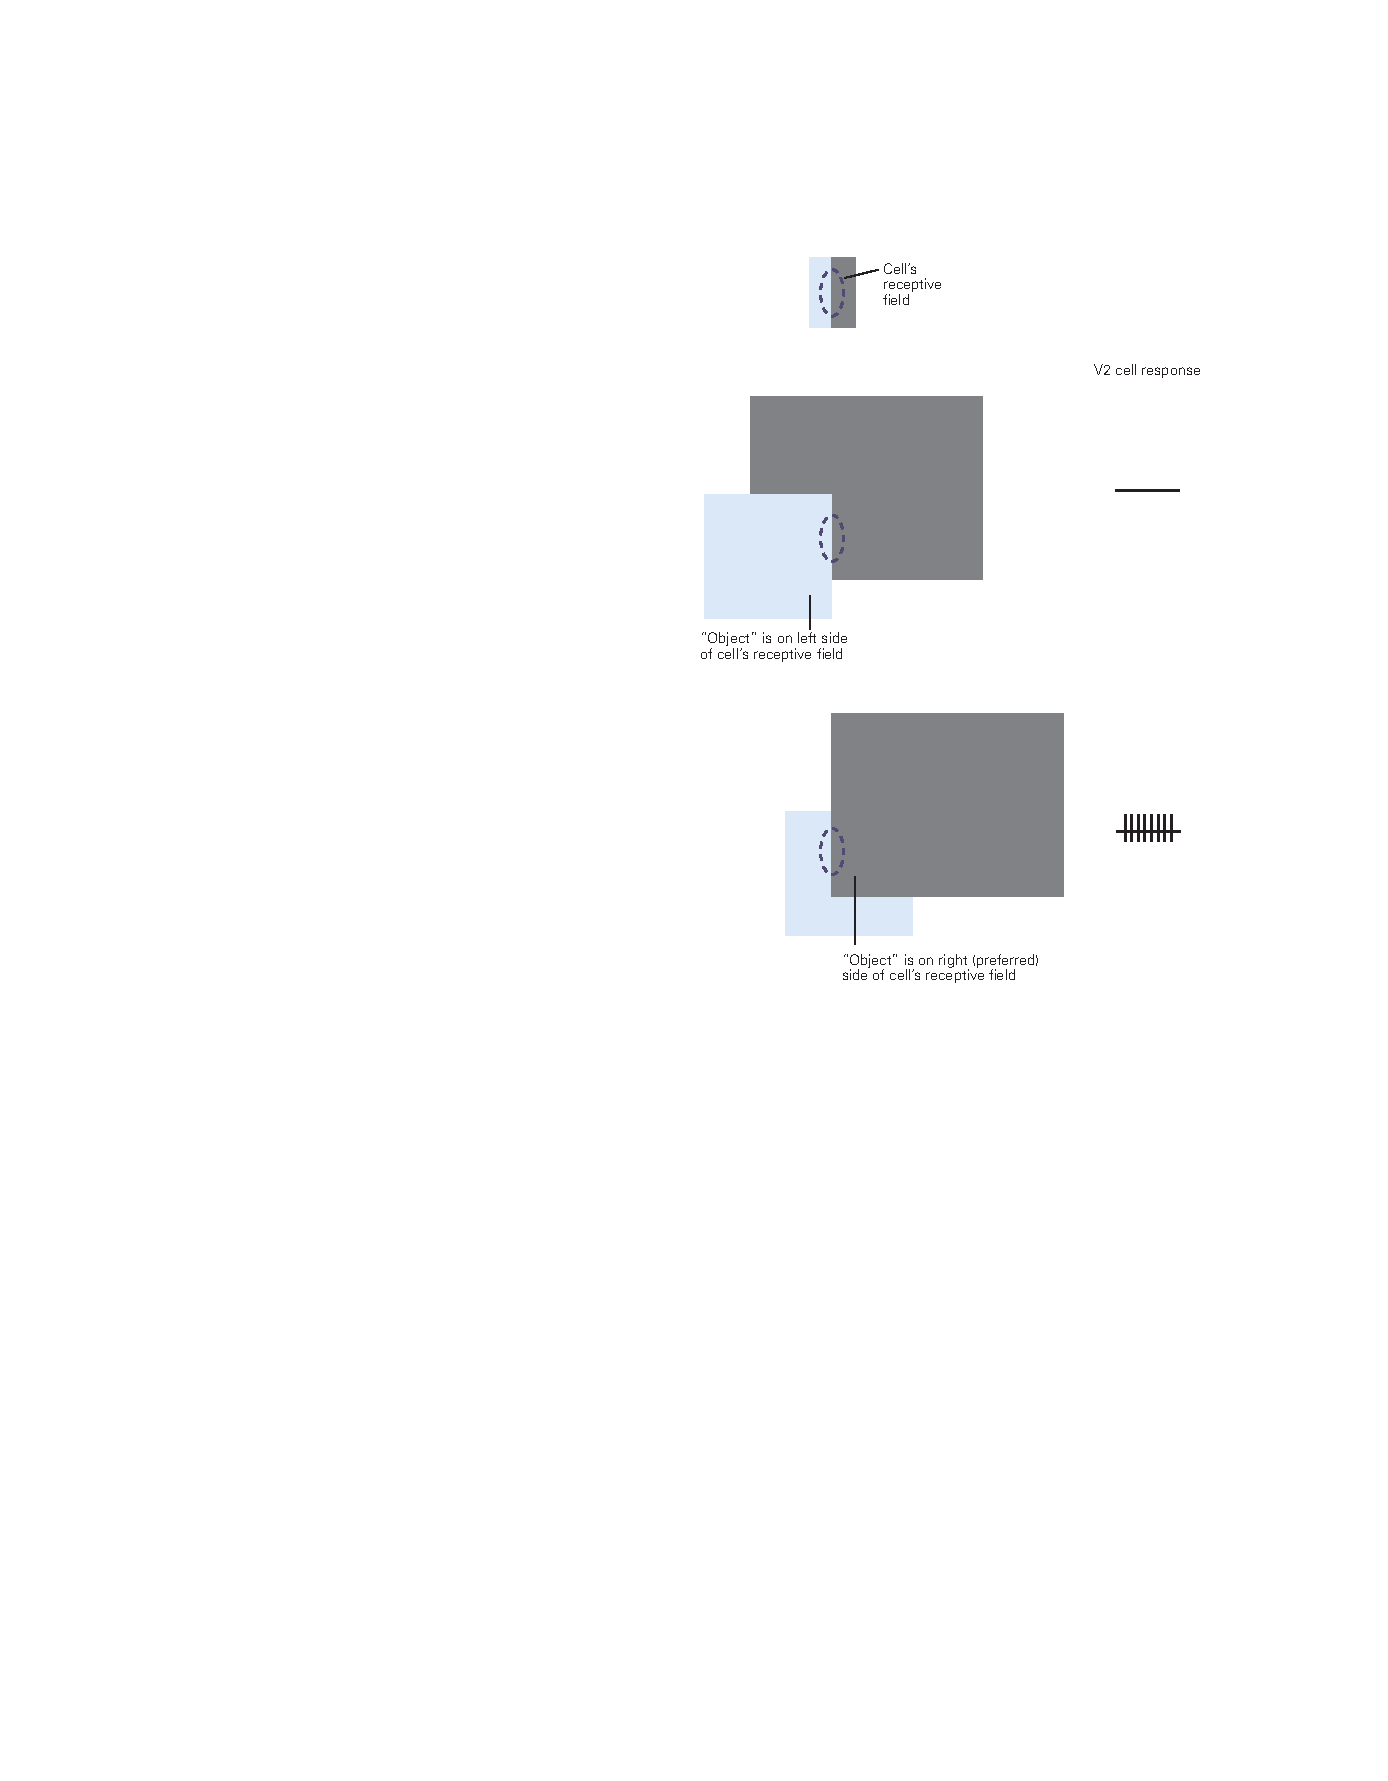
\includegraphics[width=0.75\linewidth]{chap23/fig_23_9}
	\caption{边界所有权。
		区域 V2 中的细胞对整个目标的边界敏感。
		尽管细胞感受野内的两个矩形的局部对比度相同,但只有当边界是位于感受野首选侧完整矩形的一部分时,细胞才会响应~\cite{zhou2000coding}。}
	\label{fig:23_9}
\end{figure}



\section{局部运动线索定义目标轨迹和形状}

主要的视觉皮层确定目标运动的方向。
神经元中的方向选择性可能涉及感受野不同侧面区域的顺序激活。


如果以适当的速度移动的物体首先遇到具有长响应潜伏期的神经元感受野的区域,然后进入逐渐较短的潜伏期的区域,则整个接受场的信号将同时到达细胞,而神经元将剧烈发射。
如果目标朝相反的方向移动,则来自不同区域的信号不会汇总,并且细胞可能无法达到触发阈值(图~\ref{fig:23_10})。


\begin{figure}[htbp]
	\centering
	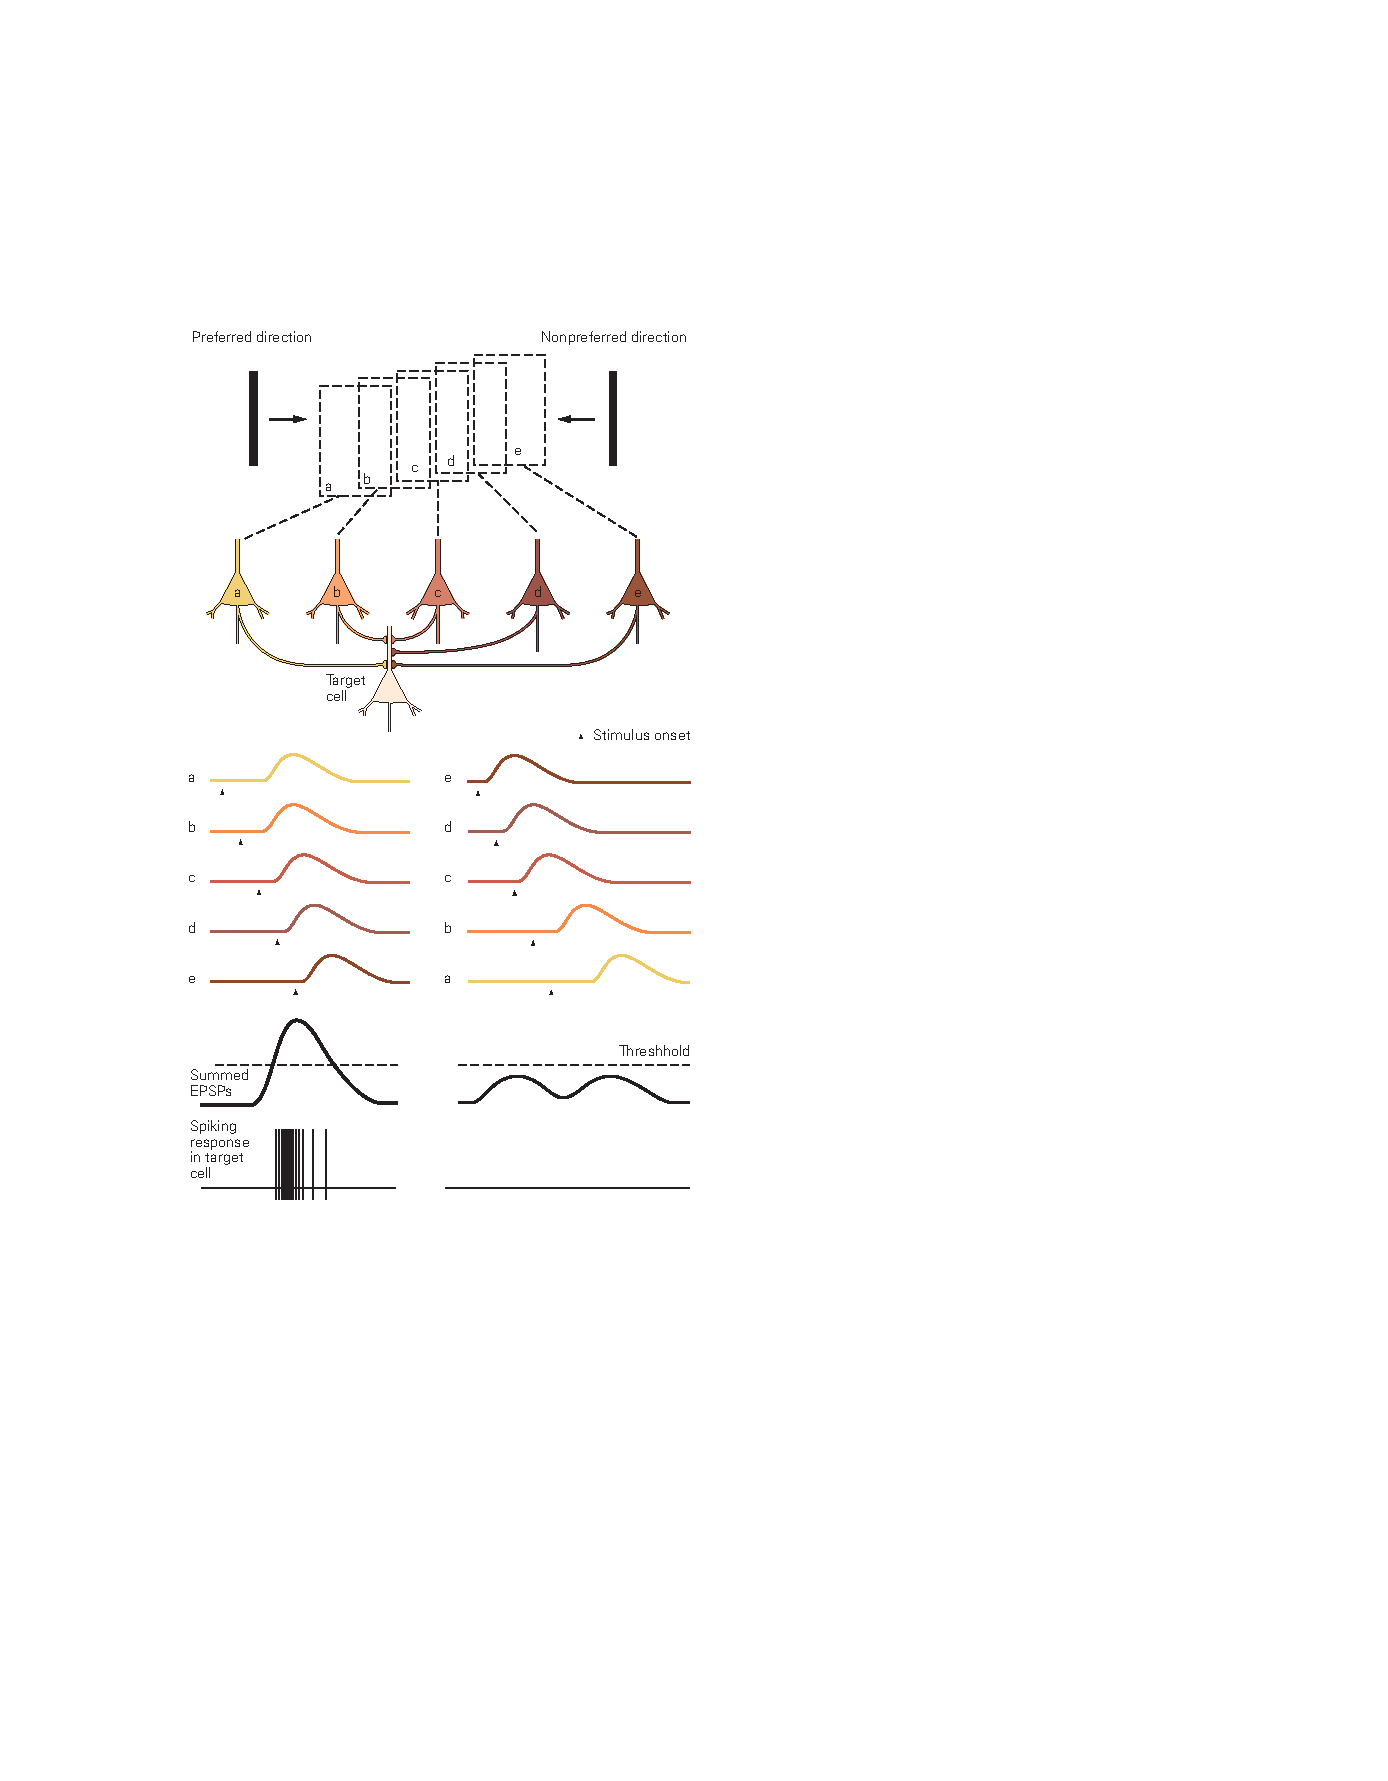
\includegraphics[width=0.7\linewidth]{chap23/fig_23_10}
	\caption{运动的方向选择性。
		神经元对运动方向的选择性取决于突触前神经元相对于刺激开始的反应潜伏期。
		突触前神经元 $a$ 和 $b$ 的反应潜伏期比神经元 $d$ 和 $e$ 的反应潜伏期稍长。
		当刺激从左向右移动时,神经元 $a$ 和 $b$ 首先被激活,但由于它们的反应潜伏期较长,它们的输入到达目标神经元与神经元 $d$ 和 $e$ 的输入叠加,叠加的输入导致神经元激活。
		相反,向左移动的刺激产生的信号会在不同时间到达目标神经元,因此不会达到细胞的放电阈值\cite{priebe2008inhibition}。}
	\label{fig:23_10}
\end{figure}


在视觉途径的早期,对物体运动的分析受感觉神经元的接受场的大小的限制。 
即使在最初的皮层区域初级视觉皮层和 V2 中,神经元的接受场也很小,并且可能仅包含一个物体的一小部分。 
然而,最终必须将有关目标离散方面运动的方向和速度集成到整个目标运动的计算中。 
这个问题比人们预期的要困难得多。


如果一个人观察到一个复杂的形状穿过小孔,则光圈内物体边界的一部分似乎沿垂直于边界方向的方向移动(图~\ref{fig:23_11}a)。 
如果线的末端不可见,则无法检测到线的真实运动方向。 
如果线的图像沿着垂直于其方向的轴缓慢移动,或者沿斜轴迅速移动,则该线的图像看起来相同。
这是初级视觉皮层神经元的接受场提出的难题。 
视觉系统的解决方案是假设轮廓的运动垂直于其方向。 
因此,首先将一个物体呈现给视觉系统,其中无数小块具有不同方向的边界,所有这些似乎都以不同的方向和不同速度移动(图~\ref{fig:23_11}a)。


\begin{figure}[htbp]
	\centering
	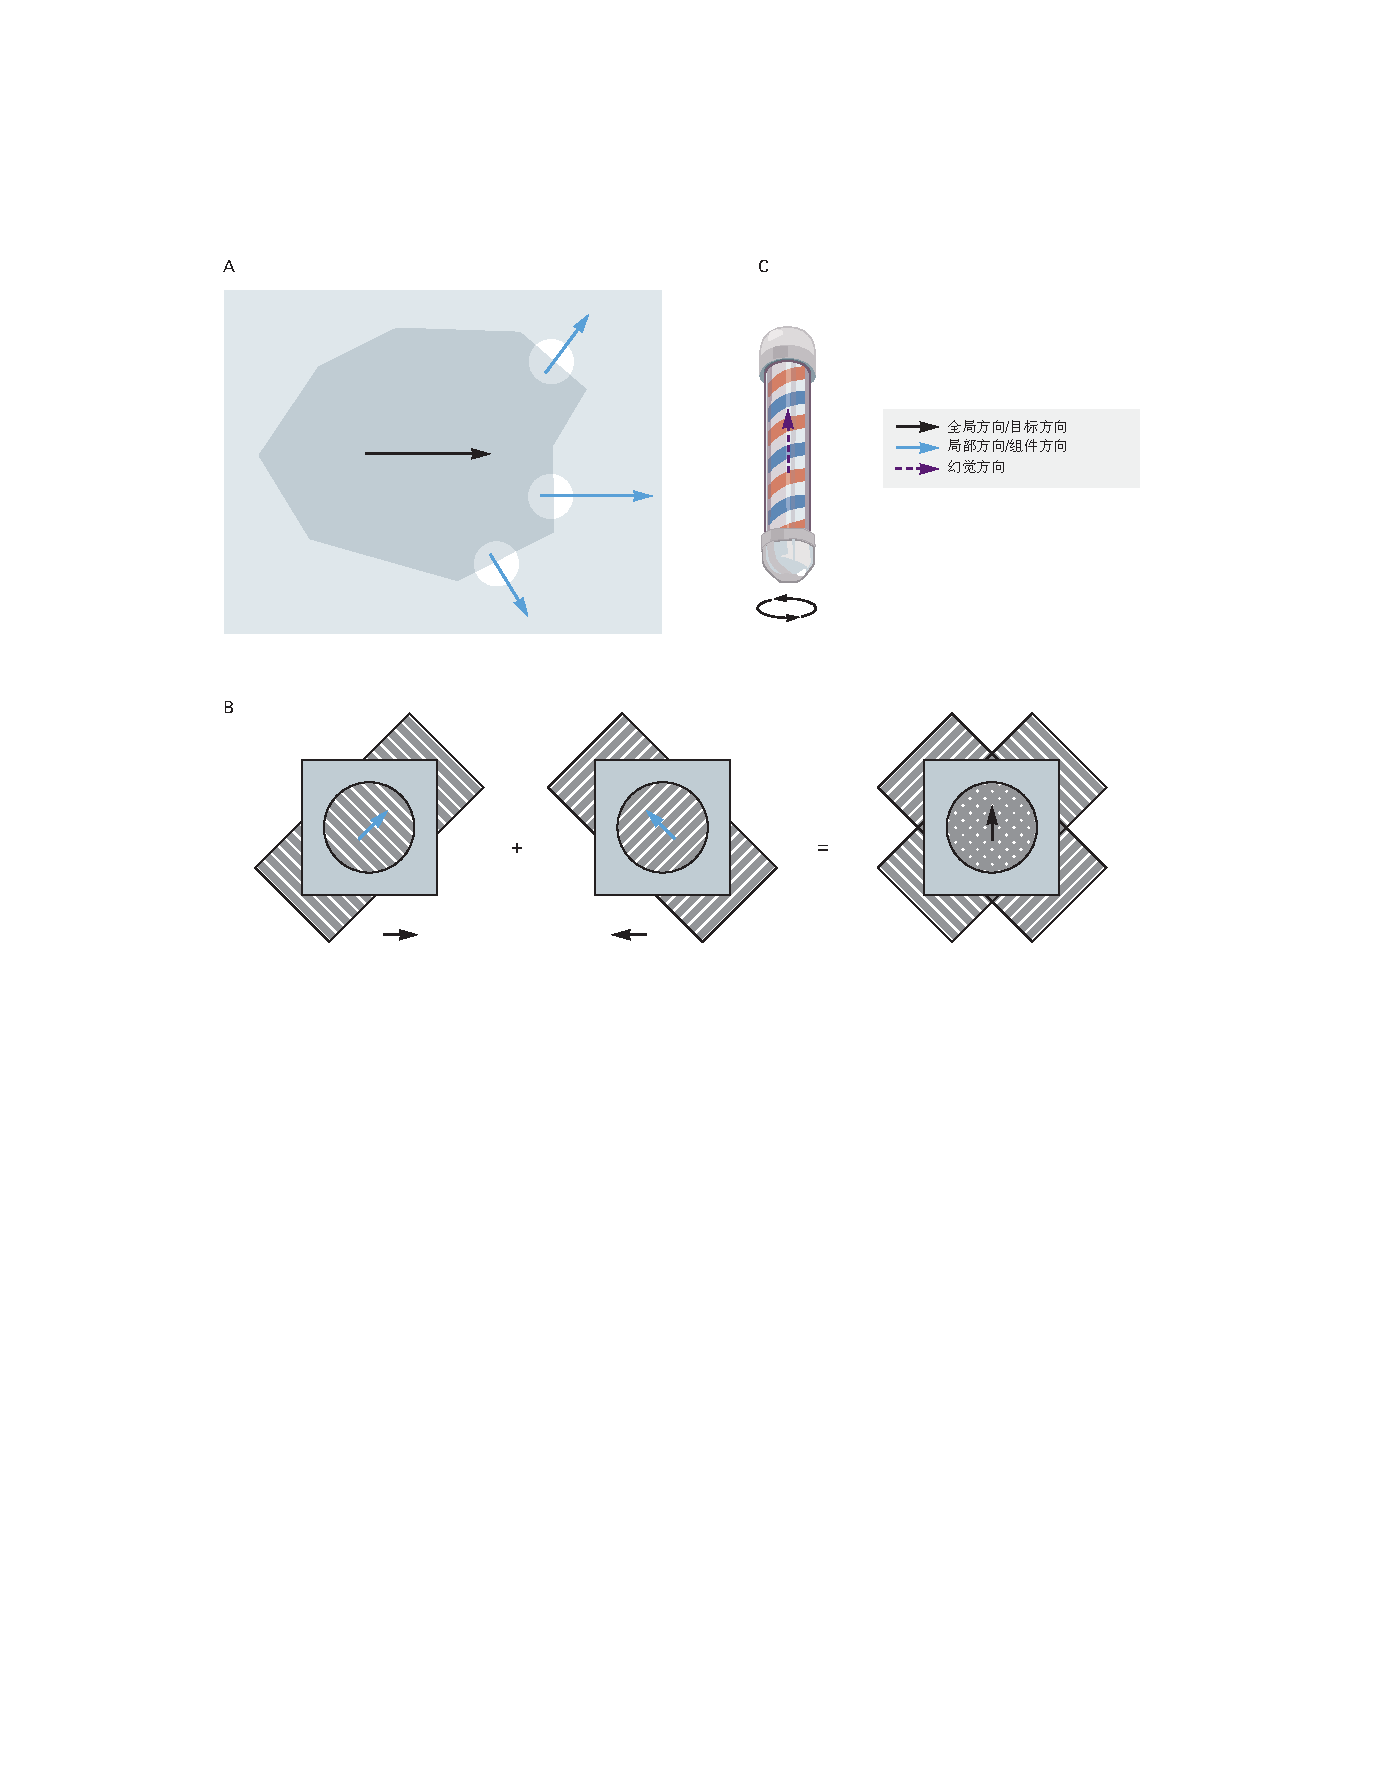
\includegraphics[width=1.0\linewidth]{chap23/fig_23_11}
	\caption{孔径问题和理发杆错觉。
		\textbf{A.} 虽然一个物体在一个方向上移动,但当通过一个小孔径观察时,每个组件边缘似乎都在垂直于它的方向的方向上移动。
		视觉系统必须将这些局部运动信号整合到对移动物体的统一感知中。
		\textbf{B.} 光栅用于测试神经元是否对局部运动信号或全局运动信号敏感。
		当光栅叠加并沿不同方向独立移动时,人们不会看到两个光栅相互滑过,而是看到格子图案在一个中间方向上移动。
		猴子中颞区的神经元对这种整体运动而不是局部运动有响应。
		\textbf{C.} 运动感知受场景分割线索的影响,如理发师杆错觉所示。
		尽管杆子围绕其轴旋转,但由于理发杆外壳的全局垂直矩形环绕,人们会认为条纹是垂直移动的。}
	\label{fig:23_11}
\end{figure}


确定目标的运动方向需要解决多个提示。
可以通过将一个栅格放在另一个上方并将两个方向移动到不同方向上,可以很容易地证明这一点。
所得的棋盘格态似乎在单个光栅的轨迹之间沿中间方向移动(图~\ref{fig:23_11}b)。
这种感知取决于光栅的相对对比和光栅重叠的区域。
由于相对对比很大,光栅似乎相互滑动,朝着他们的各个方向移动,而不是朝着共同的方向移动。


感知方向的一个重要决定因素是场景分割,将移动元素分离到前景和背景。
在具有移动目标的场景中,分割不是基于方向的本地提示。
相反,对方向的感知取决于场景细分。
理发界的幻觉提供了另一个例子,说明了全球关系在简单属性的感知上占主导地位。
旋转条纹被认为是沿极长轴垂直移动的(图~\ref{fig:23_11}c)。
视野中运动的感知使用了一种复杂的算法,该算法将本地运动信号的自下而上分析与自上而下的场景分割相结合。


在颞中部区域(\textit{内侧颞叶}或 V5 区域)中观察到了猴子中局部运动信号的整合,该区域是专门运动的区域。
该区域的神经元可以选择整体模式的特定运动方向,而不是模式的单个组成部分。
这种对整体模式的依赖性也可以在理发量效应中与感知方向的响应的对应关系中看到。



\section{上下文决定视觉刺激的感知}

\subsection{亮度和颜色感知取决于上下文}

视觉系统通过比较来自视野的不同部分到达的光来测量目标的表面特征。
结果,对亮度和颜色的感知高度取决于上下文。
实际上,感知到的亮度和颜色可能与物体的物理特性所期望的完全不同。
同时,即使照亮它们的光的亮度和波长分布从天然光到人造光,从阳光到阴影,或从黎明到中午,即使光的亮度和波长分布也会显得相似(图~\ref{fig:23_12}A)。


\begin{figure}[htbp]
	\centering
	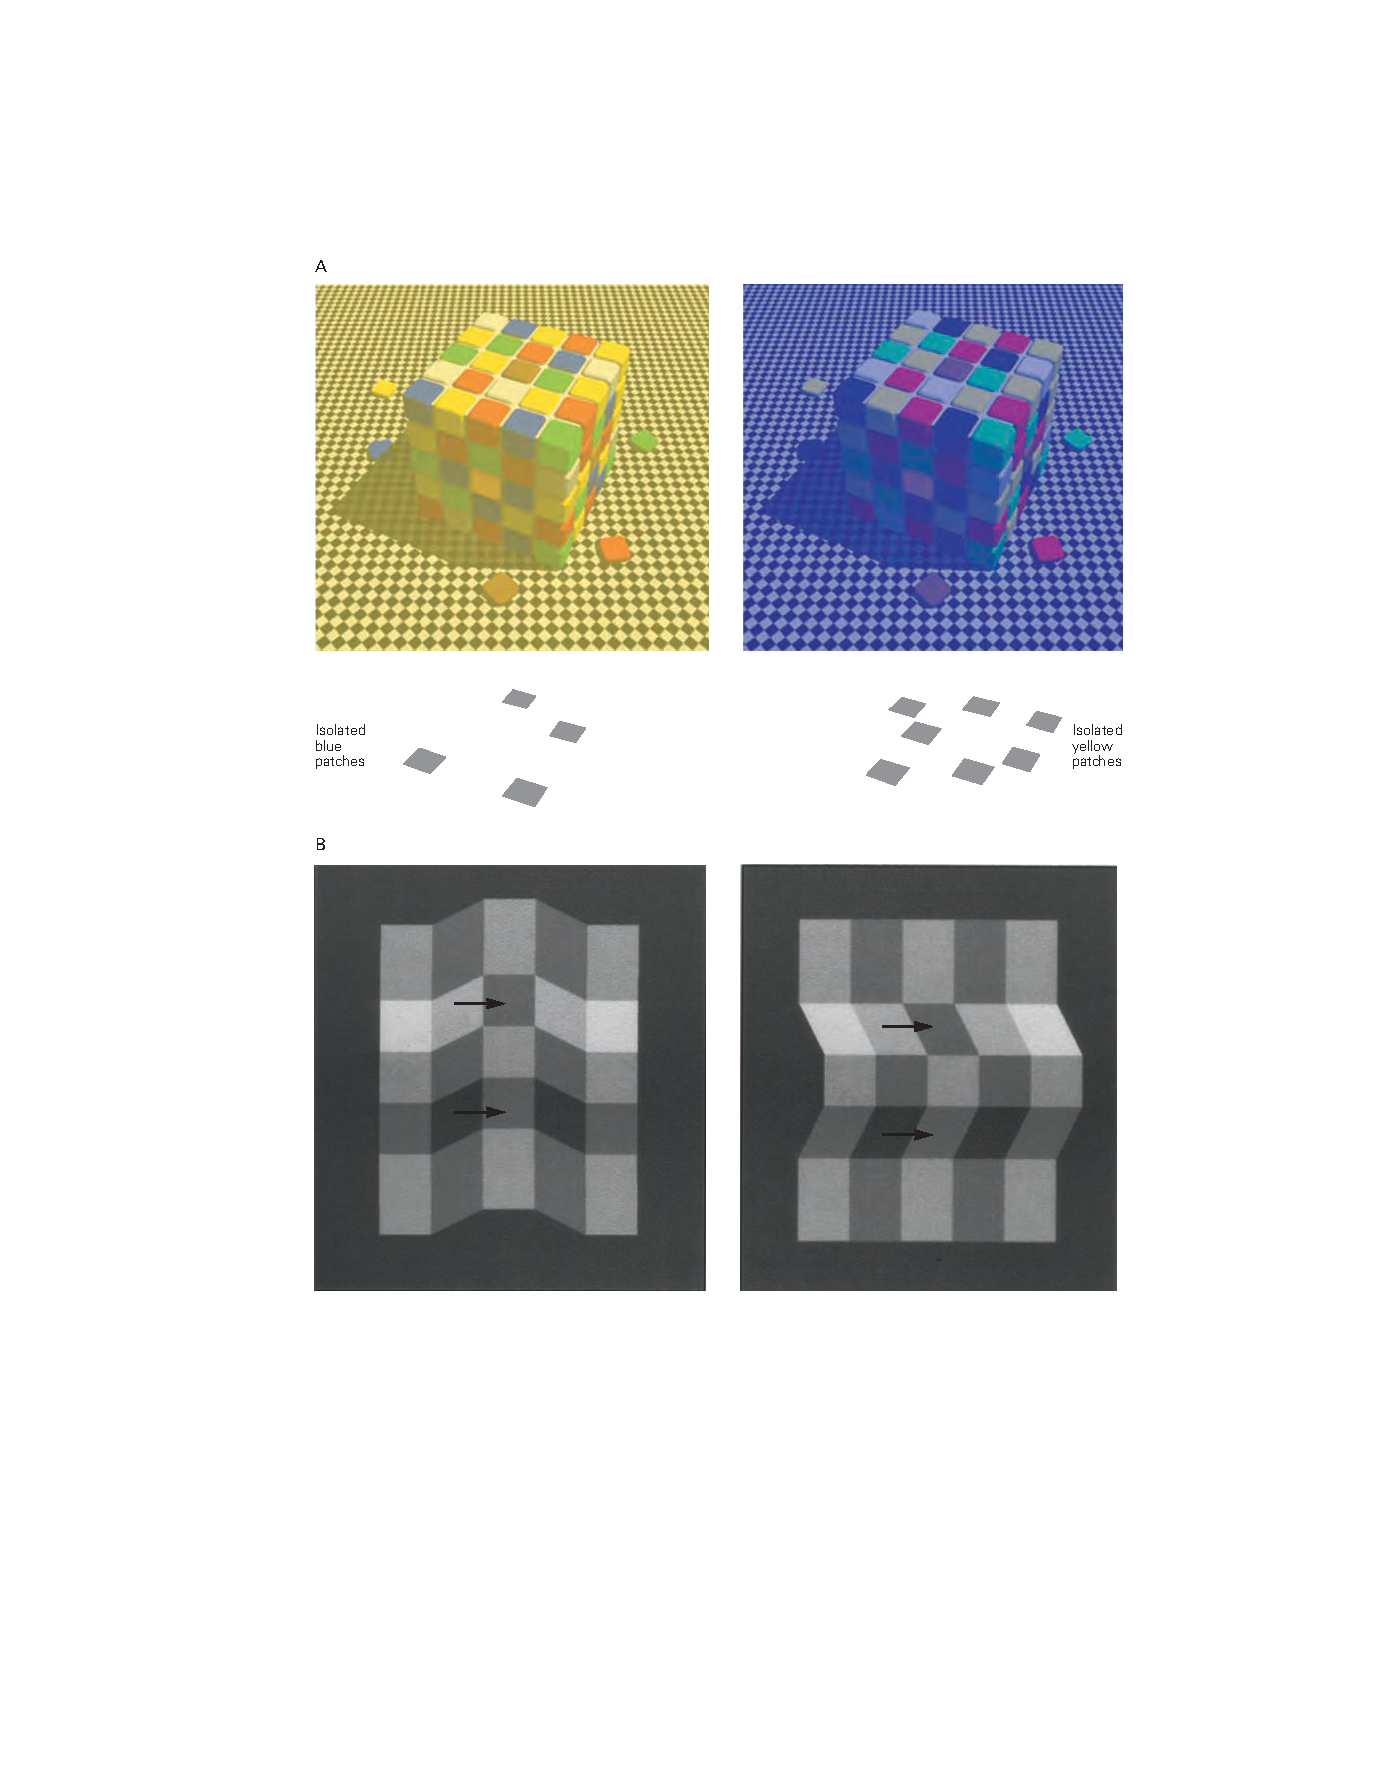
\includegraphics[width=1.0\linewidth]{chap23/fig_23_12}
	\caption{颜色和亮度感知取决于上下文提示。
		\textbf{A.} 感知的表面颜色在不同的光照条件下保持相对稳定,因此从表面反射的光的波长也会发生变化。
		尽管来自两组表面的光波长非常不同,但左右立方体上的黄色方块看起来很相似。
		事实上,如果将左侧立方体顶部的蓝色方块和右侧立方体顶部的黄色方块与其上下文方块隔离开来,它们的颜色看起来是相同的。
		\textbf{B.} 亮度感知也受三维形状的影响。
		箭头指示的四个灰色方块都具有相同的亮度。
		左图中的视亮度相似,而右图中的视亮度不同。
		这是因为视觉系统有一个固有的期望,即照明来自上方(太阳相对于我们的位置),因此认为右侧插图中褶皱下方的表面比上方相同亮度的表面更亮\cite{adelson1993perceptual}。}
	\label{fig:23_12}
\end{figure}


当我们四处移动或随着环境照明的变化,物体的视网膜图像(大小,形状和亮度)也会发生变化。
然而,在大多数情况下,我们不认为目标本身正在改变。
当我们从光明的花园转移到一个昏暗的房间时,到达视网膜的光强度可能会有所不同。
无论是在房间的昏暗照明中,还是在阳光的眩光中,我们仍然看到一件白色衬衫,如白色和红色的领带。
同样,当朋友向你走去时,她被认为越来越近。
即使视网膜上的图像确实扩大,您也不会认为她会变得更大。
我们将物体的大小和颜色感知为常量的能力再次说明了视觉系统的一个基本原理:
它不像相机那样被动地记录图像,而是使用视网膜的瞬时和可变刺激来构建稳定的三维世界。


上下文影响的另一个例子是颜色诱导,其中颜色在一个区域中的出现在相邻区域中转向颜色。
形状在表面亮度的感知中也起着重要作用。
由于视觉系统假设照明来自上方,因此折叠表面上的灰色斑块躺在表面的顶部或底部,即使它们实际上是相同的灰色阴影(图~\ref{fig:23_12}b),它们也会大不相同(图~\ref{fig:23_12}b)。


视觉皮层中某些神经元的反应与感知的亮度相关。
大多数视觉神经元对表面边界有反应。
视网膜神经节细胞和统一神经元的感受野的中心仪结构适合捕获边界。
大多数此类细胞对表面的内部部分没有反应,因为均匀的内部内部没有产生跨感受野的对比梯度。
但是,一小部分神经元确实对表面的内部,信号局部亮度,质地或颜色做出了反应,这些神经元的反应受到情境影响。
即使在感受野内的表面亮度保持固定时,细胞的亮度也会随着细胞接受场外面的亮度的变化而变化。


由于大多数神经元对表面边界的反应,而不是对均匀亮度的区域的反应,因此视觉系统通过有关表面边缘的对比度的信息来计算表面的亮度。
大脑对边界信息表面质量的分析称为感知填充。
如果将黑盘和周围明亮区域之间的边界固定几秒钟,则磁盘将以与周围区域相同的亮度“填充”。
之所以发生这种情况,是因为仅当眼睛或刺激移动时,响应边缘的细胞就会发射。
他们逐渐停止响应稳定的图像,不再向边界的存在发出信号。
磁盘内具有感受野的神经元逐渐开始以类似于周围区域具有接受场的方式的方式响应,表现出其接受场特性的短期可塑性。


尽管在不同的照明条件下,从物体反射的光的波长分布差异很大,但目标的颜色总是显得或多或少。
要识别一个目标,我们必须知道其表面的属性,而不是不断变化的反射光的属性。
因此,目标颜色的计算比分析反射光谱更为复杂。
为了确定表面的颜色,必须确定入射光的波长分布。
在没有这些信息的情况下,可以通过确定场景中不同表面的波长平衡来估算表面颜色。
如果感知的颜色保持恒定,则 V4 中的一些神经元对不同的照明波长的反应类似。
通过对广泛表面的光响应,这些神经元可以选择表面颜色而不是波长。



\subsection{感受野属性取决于上下文}

局部和全球效应之间的区别 - 在感受野中发生的刺激与超越刺激之间的区别在于如何定义接受场本身的问题。
由于视觉皮层神经元的接受场的原始表征没有考虑到上下文的影响,因此一些研究人员现在区分“经典”和“非经典”接受场。


但是,即使对感觉接受场的最早描述也可以从狭义定义的接受场外面的感觉表面的某些部分影响。
1953年,\textit{史蒂文$\cdot$库夫勒}在对视网膜神经节细胞的感受野特性的开创性观察中,指出:“不仅可以通过视网膜照明来真正设置响应的区域 同样,通过对神经节细胞的抑制或兴奋性影响,所有显示功能连接的区域。
这很可能涉及与神经节细胞有些遥远的区域,并且本身不会设置排放。”


更有用的区别与神经元对简单刺激(例如短线段)的响应与对具有多个组分的刺激的响应进行了对比。
即使在主要的视觉皮层中,神经元也是高度非线性的。
他们对复杂刺激的反应无法从对视野周围不同位置的简单刺激的反应中预测。
相反,它们对本地特征的响应取决于嵌入功能的全局上下文。
上下文影响在中层视觉处理中普遍存在,包括轮廓集成,场景分割以及目标形状,目标运动和表面属性的确定。



\section{皮层连接、功能架构和感知密切相关}

中层视觉处理需要在整个视野中共享信息。
主要视觉皮层中的互连与该区域功能结构的关系表明该回路介导了轮廓积分。


皮层回路包括由平行于皮层表面的锥体神经元的轴突形成的远程水平连接的丛。
水平连接都存在于大脑皮层的每个区域中,但是它们的功能在一个区域到下一个区域而异,具体取决于每个区域的功能架构。
在视觉皮层中,这些连接介导了相似特异性的方向列之间的相互作用,从而在大面积的视觉皮层上集成了信息,这代表了视野的大广阔(见图~\ref{fig:21_16})。


这些水平连接链接神经元相似但代表视野中遥远位置的神经元的事实表明,这些连接在轮廓积分中起作用。
轮廓整合和轮廓显著性的相关特性反映了良好延续的格式塔原理。
两者都是由初级视觉皮层中的水平连接介导的(见图~\ref{fig:23_6})。


对视觉空间整合至关重要的皮层连接的最终特征是高阶皮层区域的反馈预测。
反馈连接与起源于丘脑或皮层加工的早期阶段的前馈连接一样广泛。
这些反馈预测的功能知之甚少。
他们可能在调解自上而下的关注,期望和感知任务的影响方面发挥作用,所有这些都会影响皮层处理的早期阶段。



\subsection{感知学习需要皮层连接的可塑性}

眼部占主导地位的突触连接仅适用于在开发的关键时期(第~\ref{chap:chap49}~章)。
这表明视觉皮层神经元的功能特性是在成年中固定的。
然而,皮层神经元的许多特性在一生中仍然可变。
例如,视网膜病变后可能发生视觉皮层的变化。


当局灶性病变发生在两个视网膜上的相应位置时,最初被剥夺了视觉输入的皮层图的相应部分(称为病变投影区)。
然而,在几个月的时间里,该区域内的细胞的接受场从视网膜的病变部分转移到了病变周围的功能区域。
结果,视网膜病变部分的皮层表示,周围区域的皮层表示(图~\ref{fig:23_13})。


\begin{figure}[htbp]
	\centering
	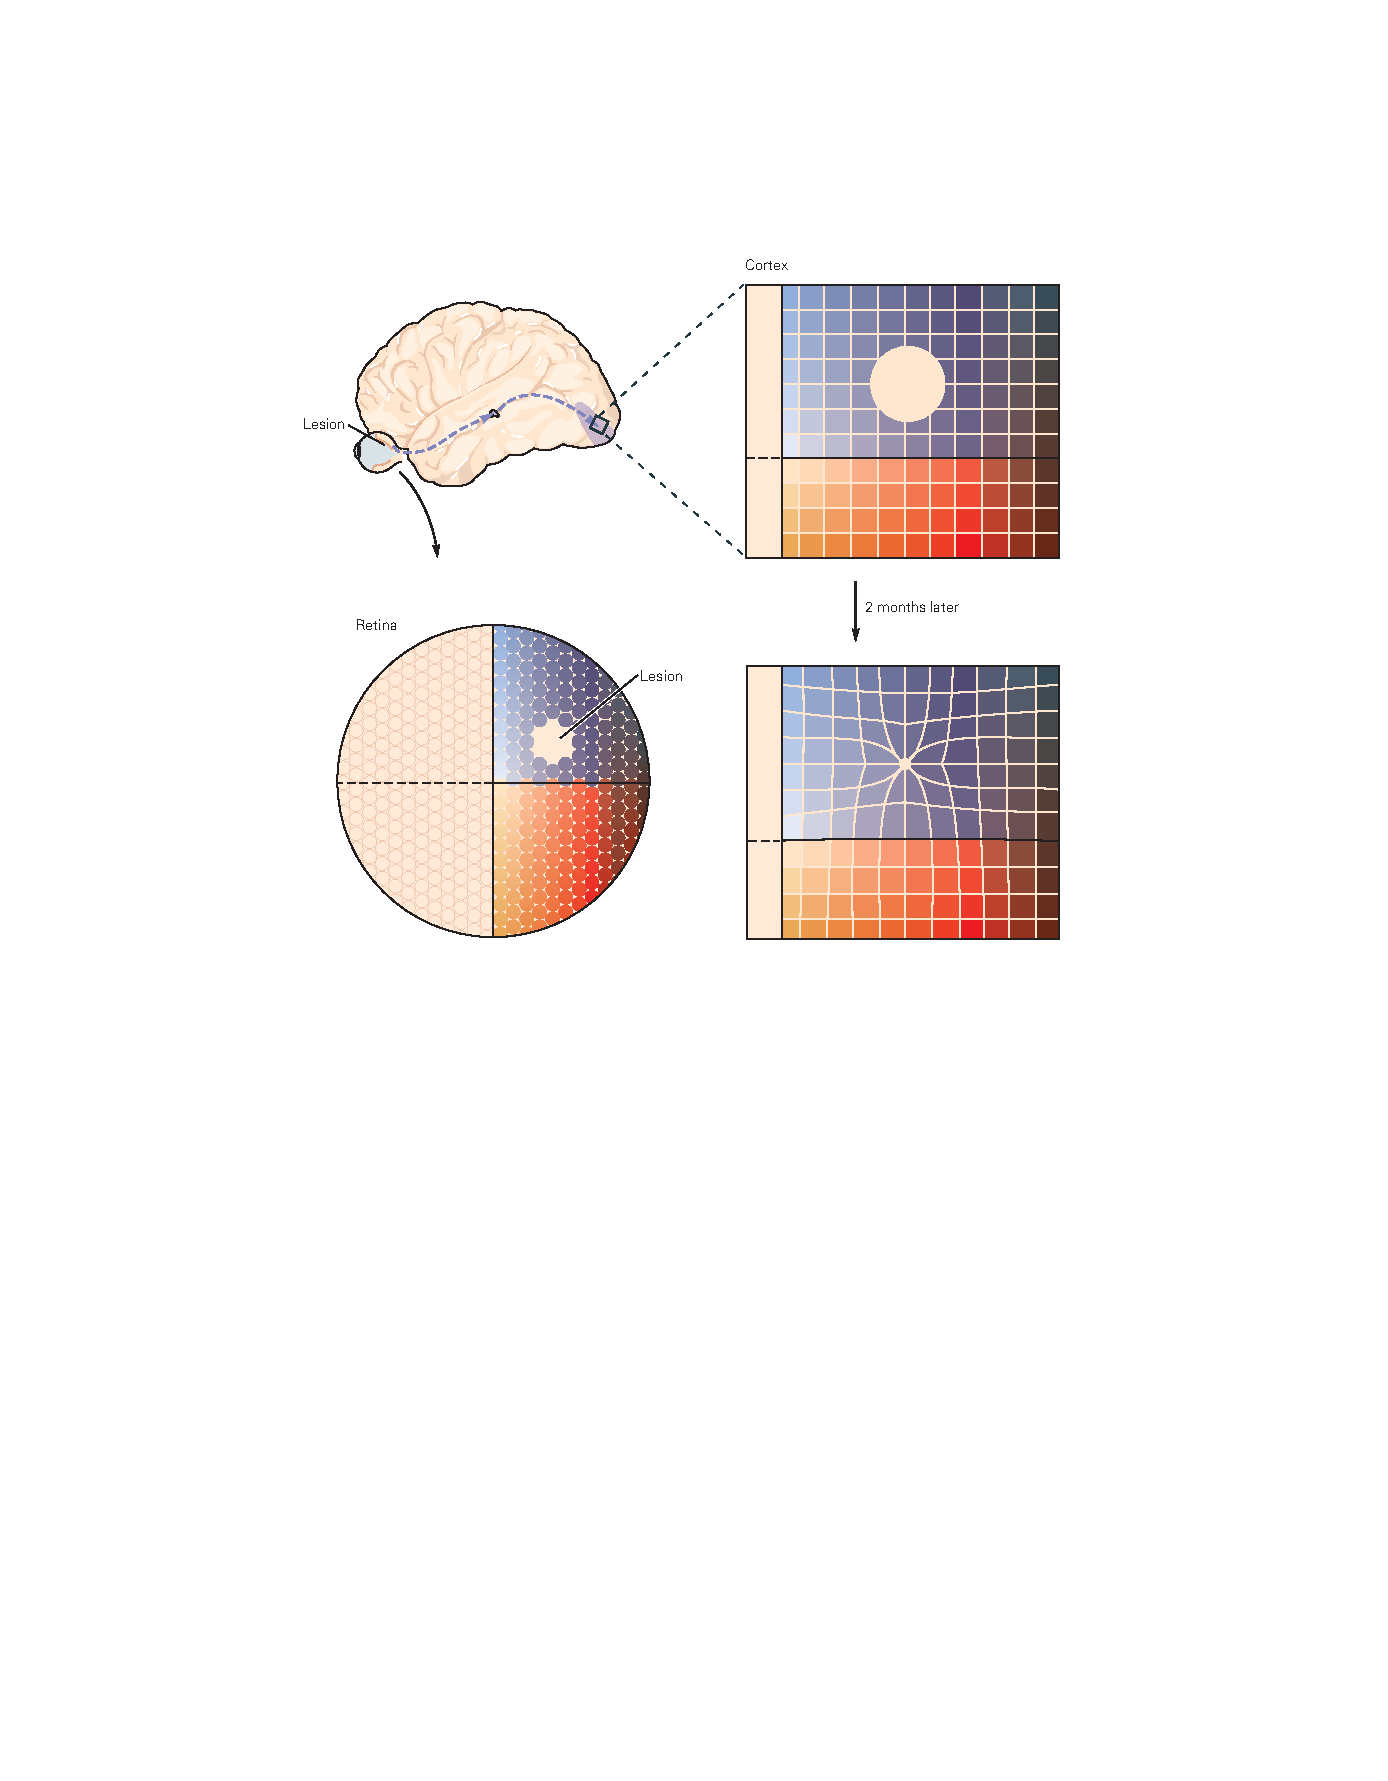
\includegraphics[width=1.0\linewidth]{chap23/fig_23_13}
	\caption{成人皮层的可塑性。
		当双眼的相应位置受损时,接收来自受损区域输入的皮层区域(病变投射区)最初是沉默的。
		病变投射区神经元的感受野最终从病变区域转移到周围完整的视网膜。
		发生这种情况是因为病变投射区周围的神经元会萌发侧枝,这些侧枝与区域内的神经元形成突触连接。
		结果,视网膜受损部分的皮层表现缩小,而周围视网膜的皮层表现扩大。}
	\label{fig:23_13}
\end{figure}


皮层图和连接的可塑性不是作为对病变的反应而发展的,而是改善我们感知技能的神经机制。
视觉皮层分析的许多属性,包括立体敏锐度,运动方向和方向,随着实践而变得更加清晰。
\textit{赫尔曼$\cdot$冯$\cdot$亥姆霍兹}在1866年表示:“感官的判断可以通过经验和在各种情况下得出的训练来修改,并且可以适应新条件。
因此,人们可以在某种程度上学习以利用这种感觉的细节,否则这些感觉将避开通知,而不会有助于获得目标的任何想法。” 
这种感知学习是多种隐性学习,不涉及有意识的过程(第~\ref{chap:chap52}~章)。


感知学习涉及多次重复辨别任务,并且不需要错误反馈来提高性能。
例如,改善表现出来,例如,在目标刺激的属性或在复杂的环境中检测目标的能力差异的阈值减少。
包括主要视觉皮层在内的几个视觉皮层区域参与感知学习。


感知学习的一个重要方面是其特异性:对一项任务的训练不会转移到其他任务。
例如,在三行二等任务中,受试者必须确定三个平行线的中心位置是更接近左侧的线还是右侧的线。
重复练习后,准确响应所需的中心位置的偏移量大大减少。


学习此任务是特定于视野中的位置和线路的方向。
这种特异性表明,视觉处理的早期阶段是造成的,因为在早期阶段,接受场是最小的,视觉图最精确的,并且定向调整最清晰。
该学习也针对刺激配置。
对三线一分为二的训练不会转移到\textit{装游标的任务}任务中,其中上下文是与目标线共线的线(图~\ref{fig:23_14}a)。


\begin{figure}[htbp]
	\centering
	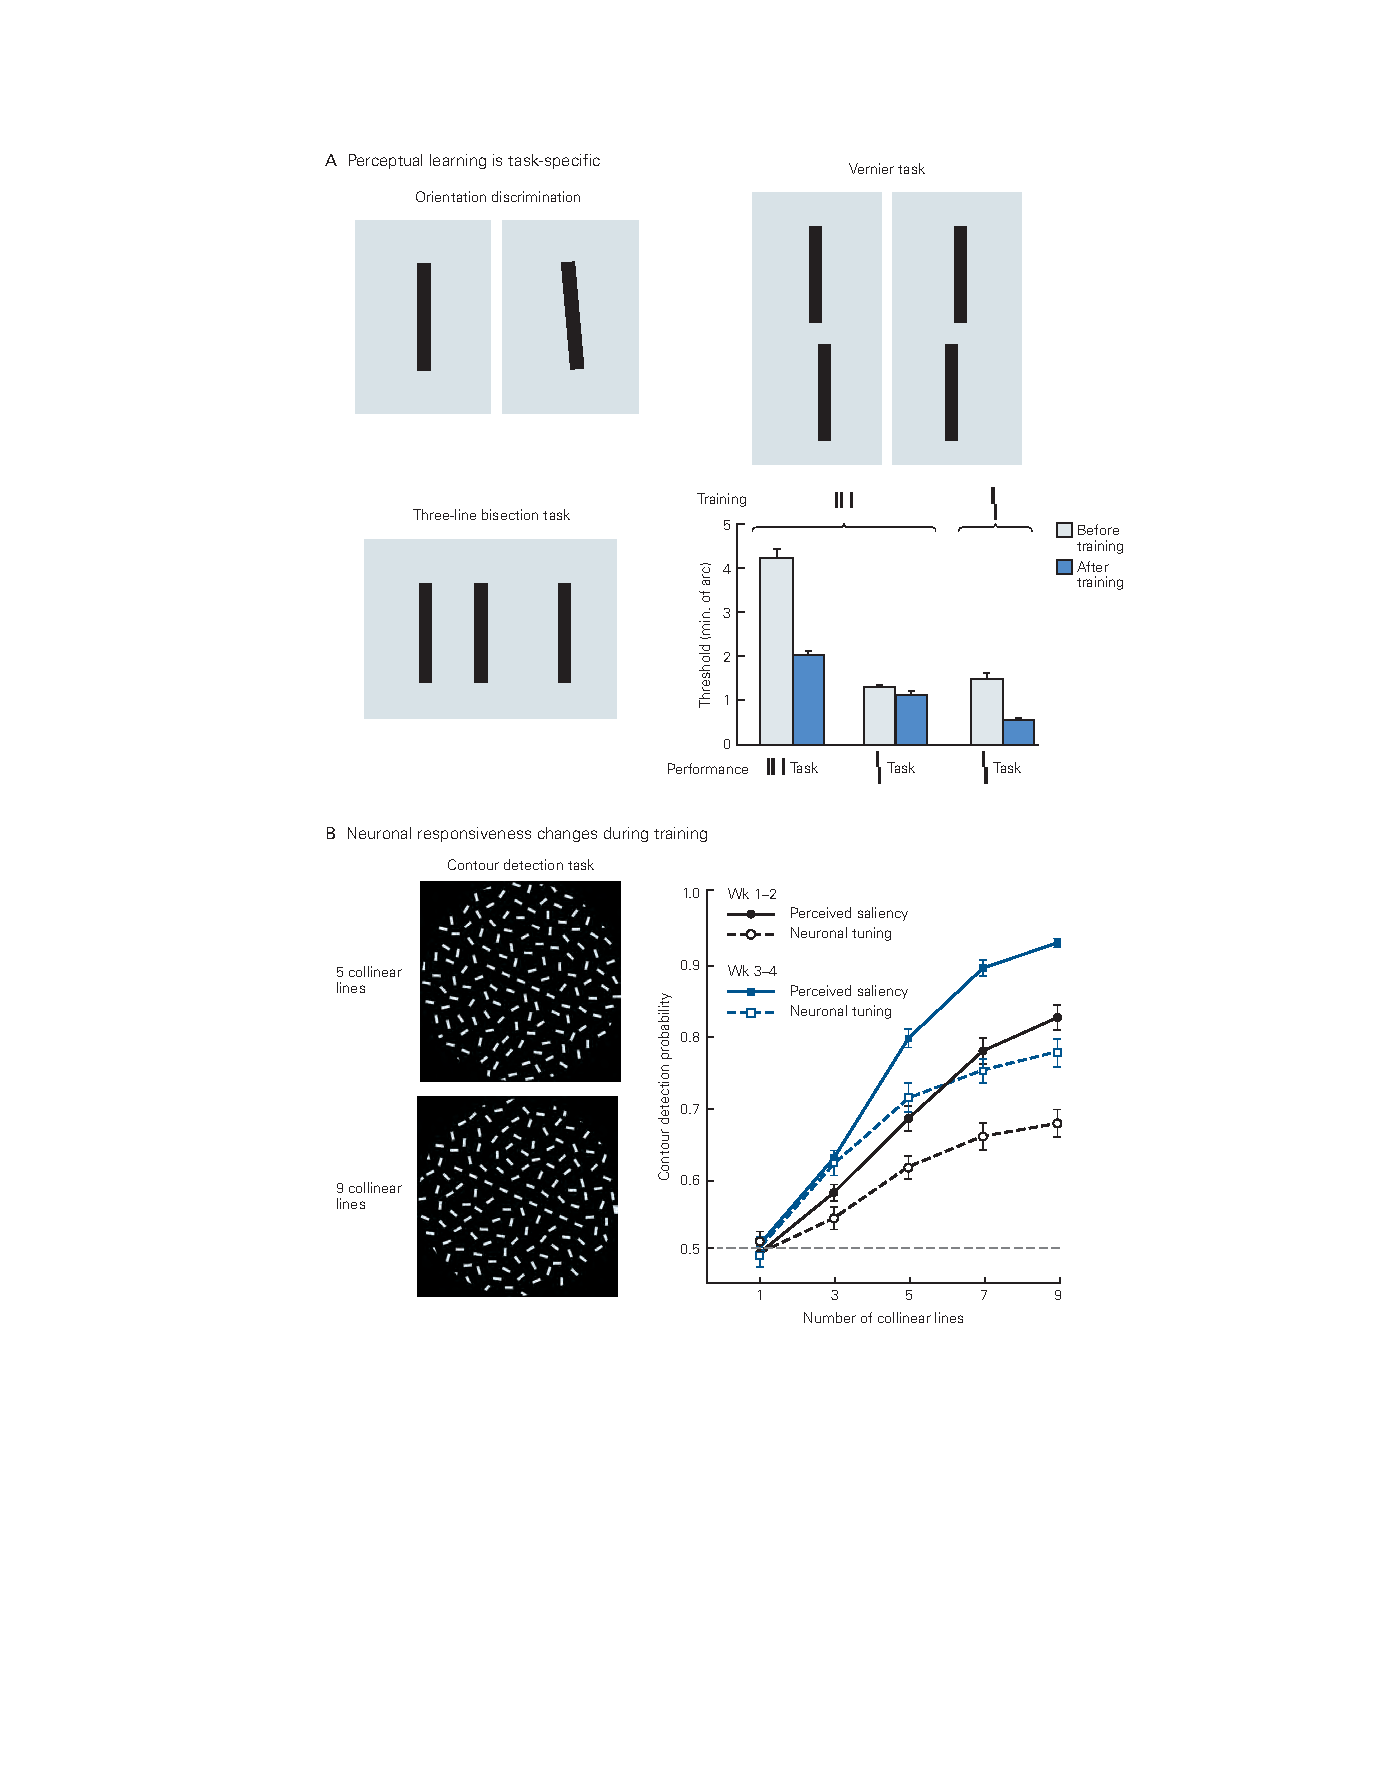
\includegraphics[width=0.89\linewidth]{chap23/fig_23_14}
	\caption{知觉学习。
		知觉学习是内隐学习的一种形式。
		通过练习,人们可以学会辨别物体在方位、位置、深度和运动方向上的微小差异。
		\textbf{A.} 这种改进被视为可靠地检测倾斜线或位于几乎共线的线(游标任务)左侧或右侧所需的变化量的减少。
		知觉学习是高度特定的,因此三线平分任务的训练会导致该任务(条形图中左侧的一对条形)的显著改进,而不会影响游标辨别任务(中央一对条形)的性能。
		然而,专门针对游标辨别的训练确实可以提高该任务的表现(右图)。
		\textbf{B.} 随着共线段数量的增加,受试者可以更容易地检测到嵌入在随机背景中的共线线段。
		随着线段数量的增加,初级视觉皮层神经元的反应相应增强。
		经过练习,分段越少的线越容易脱颖而出,随着这种改进,初级视觉皮层中的响应也增加了\cite{crist2001learning,li2008learning}。}
	\label{fig:23_14}
\end{figure}


在感知学习过程中,主要视觉皮层中神经元的响应特性以跟踪感知改善的方式。
一个例子以轮廓显著性。
通过实践,受试者可以更容易地检测嵌入在复杂背景中的轮廓。
检测随轮廓长度改善,初级视觉皮层中神经元的反应也是如此。
通过实践,受试者提高了检测到较短轮廓的能力,而初级视觉皮层神经元对较短的轮廓更敏感(图~\ref{fig:23_14}b)。



\subsection{视觉搜索依赖于视觉属性和形状的皮层表示}

诸如颜色,方向和形状之类的特征的可检测性与视觉搜索过程有关。
在复杂的图像中,某些目标脱颖而出或“弹出”,因为视觉系统以并行通路,目标和周围干扰器的特征同时处理(图~\ref{fig:23_15})。
当目标的功能复杂时,只能通过仔细检查整个图像或场景来识别目标。


\begin{figure}[htbp]
	\centering
	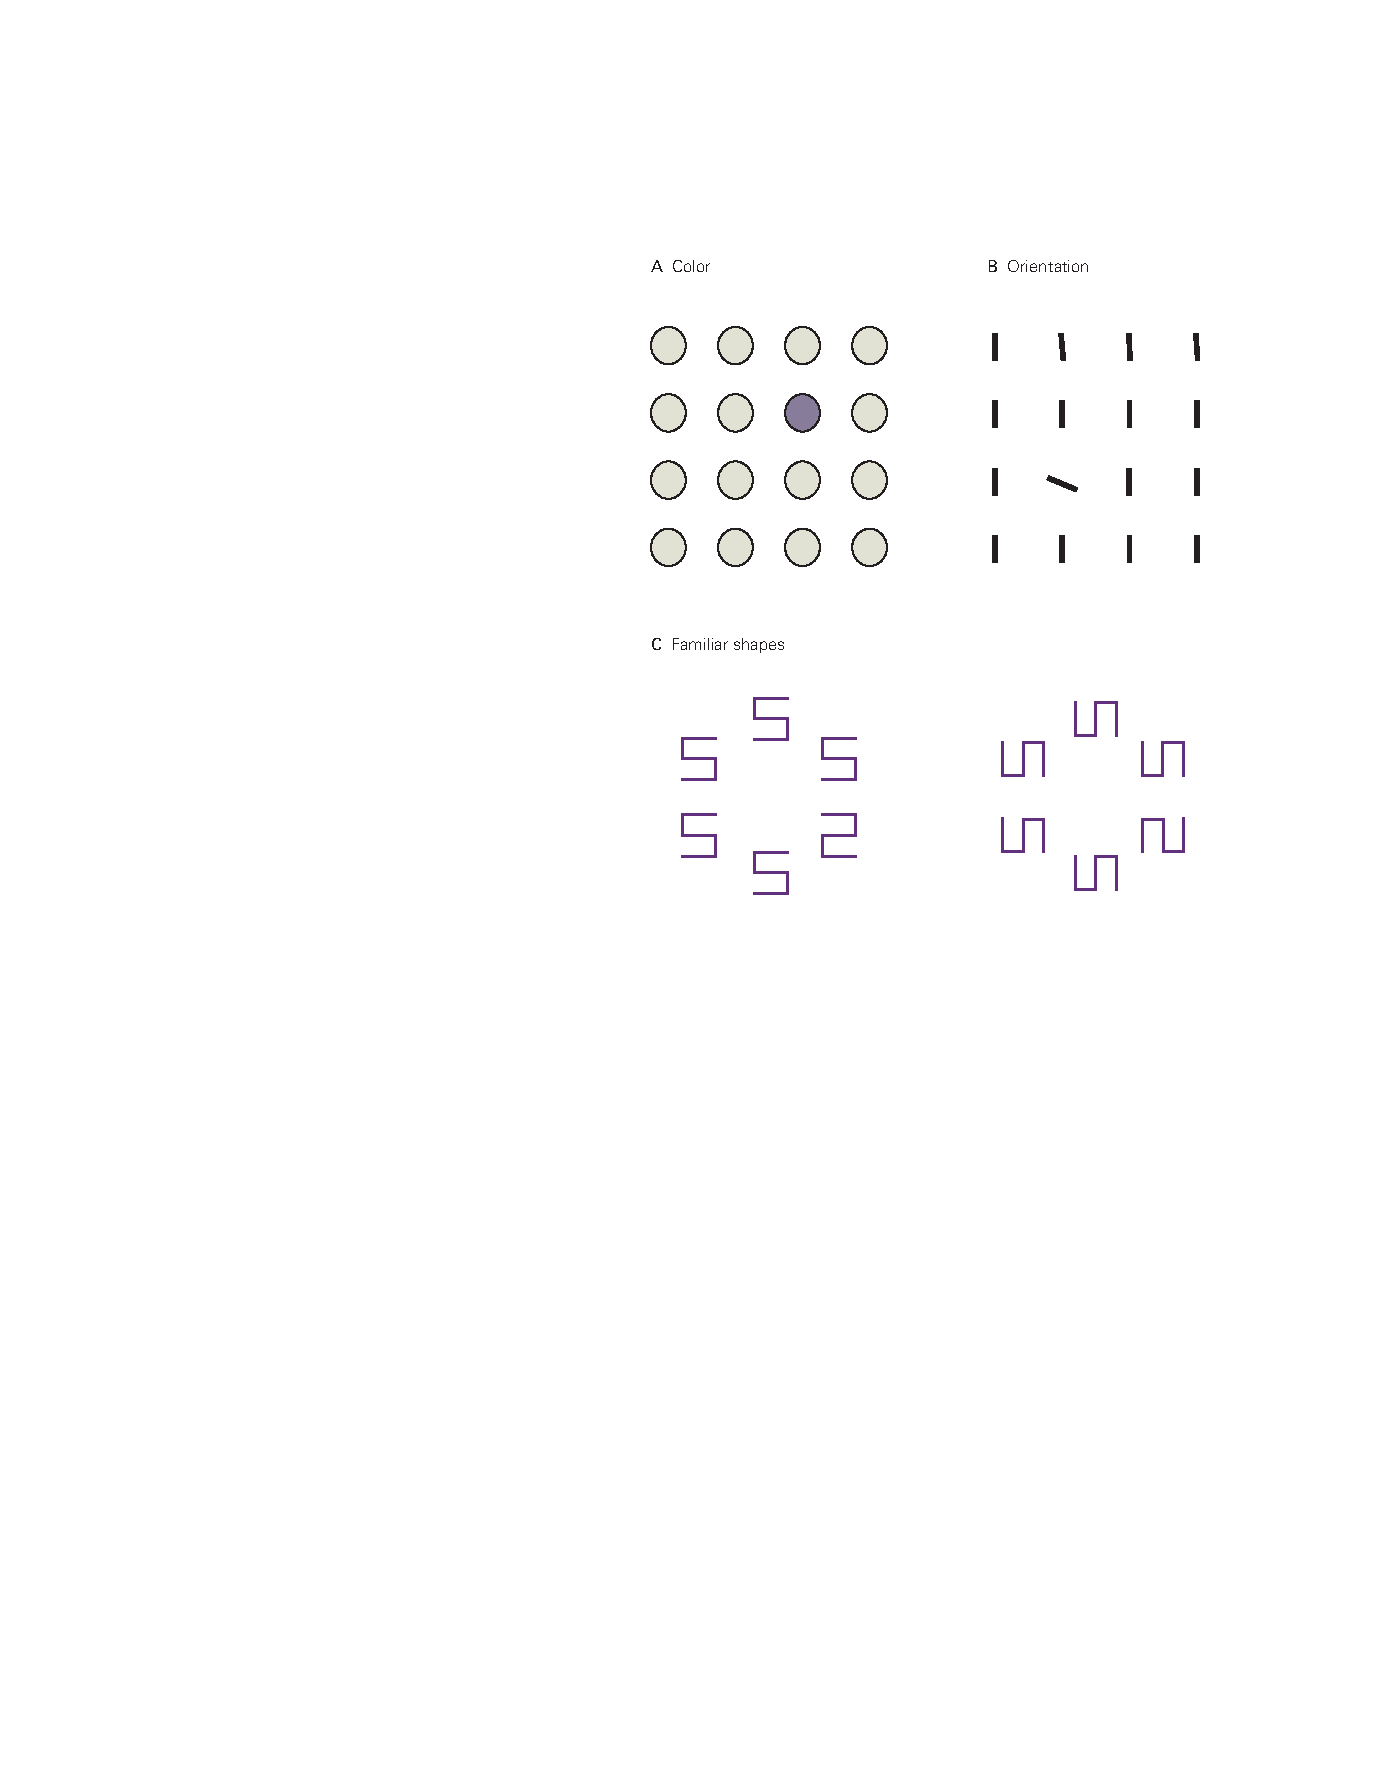
\includegraphics[width=0.75\linewidth]{chap23/fig_23_15}
	\caption{复杂图像中的一个目标在特定条件下脱颖而出。
		\textbf{A.} 弹出一个不同颜色的物体。
		\textbf{B.} 一条不同方向的线也会弹出。
		\textbf{C.} 当他们非常熟悉时,更复杂的形状会跳出来,比如数字 2 嵌入在 5 的区域中。
		将图像旋转九十度会使图形的元素难以辨认,从而更难找到与其他图形不同的图形\cite{wang1994familiarity}。}
	\label{fig:23_15}
\end{figure}


弹出现象可能会受到训练的影响。
在训练后,如果没有努力搜索,最初就无法发现的刺激。 
这种戏剧性变化的神经元相关性不确定。
对物体及其背景的特征进行并行处理是可能的,因为特征信息编码在视觉皮层多个位置的视网膜局部映射区域中。
弹出可能发生在视觉皮层的早期。
诸如数字之类的复杂形状的弹出支持的想法是,在视觉处理的早期神经元可以代表并具有选择性的形状比具有特定方向的线段更为复杂。



\subsection{认知过程影响视觉感知}

场景细分(场景分解为不同的目标)涉及到自下而上的过程的组合,这些过程遵循良好延续的格式塔规则和创造目标期望的自上而下的过程。


一种强大的自上而下的影响是空间注意力,它可以改变注意力的注意力而不会动人的眼睛动作。
空间注意力可能是面向目标的,因为注意力的焦点分布在受访目标占据的区域上,从而使视觉皮层一次分析一个目标的形状和属性。


注意机制可以解决叠加问题。
在我们可以在包含许多目标的场景中识别一个目标之前,我们必须确定哪些功能与哪些目标相对应。
我们的感觉是,我们同时识别视野中的所有目标是虚幻的。
取而代之的是,我们通过将注意力从一个转移到下一个,以快速继承目标进行序列处理。
每个分析的结果都建立了对带有许多不同目标的复杂环境的感知。
对物体识别中注意力重要性的戏剧性证明是\textit{变化盲}。
如果一个主题在同一场景的两个略有不同的视图之间迅速移动,他将无法在一个视图中发现场景中没有重要组成部分的情况而没有进行大量审查(见图~\ref{fig:25_8})。


另一个自上而下的影响是感知任务。
在视觉处理的早期阶段,同一神经元的特性随着\textit{视觉辨别}的类型而变化。
目标识别涉及一个假设检验的过程,其中将来自视网膜到达的信息与目标的内部表示。
该过程反映在研究表明,当没有视觉输入而想象场景的情况下,加工的早期阶段(例如主要的视觉皮层)会激活。



\section{亮点}

1.视觉需要将目标隔离到其背景,这是一个涉及轮廓集成和表面分割的过程。 


2.通过依靠自然形式的统计特性来简化此过程。
正如20世纪初格斯塔尔特心理学家所认可的那样,我们自然地将场景组件基于相似性,接近性和轮廓平滑度的分组(称为“良好的延续”)。


3.视觉皮层区域中的神经元具有与格式塔分组规则相辅相成的。
他们并联对场景属性进行本地和全局分析。
局部属性是视觉原始素,其中包括方向选择性,方向选择性,对比度灵敏度,差异选择性和颜色选择性。
相应的全局属性包括轮廓集成,目标运动,边界所有权,差异捕获和颜色恒定。


4.视觉特征的感知取决于上下文;
同样,神经元反应依赖上下文。
这些相互作用的基本原理是关联区域,这是每个皮层区域映射的信息位之间的相互作用模式。
关联场介导视觉皮层中的轮廓积分,但可能是整个大脑皮层加工的一般特征。
关联场的解剖基板包括由皮层金字塔细胞轴突形成的远程水平连接网络,该水平连接的长距离延伸至平行于皮层表面。 


5.不同的视觉皮层区域有助于各种全球性能,并且其开发需要区域之间的相互作用,包括自上而下的影响。
尽管人们非常强调选择性提高刺激复杂性,因为人们通过从主要视觉皮层到颞(腹侧通路)和顶侧(侧面通路)(背侧通路)皮层的区域延伸到皮层区域的层次结构,反馈连接是同等的重要性。 


6.未来的研究将在皮层加工中阐明内在,前馈和反馈皮层连接及其之间的相互作用的相对贡献。
有证据表明,神经元不是具有固定功能,而是自适应处理器,在不同的行为背景下扮演不同的功能角色。
神经元可以通过输入选择,表达与任务相关的输入并抑制任务相关的输入来介导这种功能多样性。
当异常运行时,这些功能和连通性动态可能会解释与孤独症和精神分裂症等疾病相关的感知和行为现象。

